\documentclass[a4paper,openbib,10pt]{article}
%\documentclass[a4paper,openbib,draft]{article}
%\usepackage[boxed]{algorithm}
\usepackage{afterpage}
%\usepackage{algorithmic}
\usepackage{alltt}
\usepackage{amsfonts}
\usepackage{amsmath}
\usepackage{amsthm}
\usepackage{boxedminipage}
\usepackage{calc}
\usepackage{color}
\usepackage{endnotes}
\usepackage{enumerate}
\usepackage{graphs}
\usepackage{graphicx}
\usepackage{indentfirst}
%\usepackage{ite}
\usepackage{makeidx}
%\usepackage{minitoc}
%\usepackage{multind}
%\usepackage{natbib}
%usepackage{wrapfig}

%\setlength{\textwidth}{15.7cm}
%\setlength{\textheight}{25cm}

%\setlength{\oddsidemargin}{0pt}

%\setlength{\topmargin}{0cm}
%\setlength{\headheight}{0cm}
%\setlength{\headsep}{0cm}
%\setlength{\topskip}{0cm}


%\setlength{\textwidth}{15.7cm}
%\setlength{\textheight}{24.2cm}

%\setlength{\oddsidemargin}{0pt}

%\setlength{\topmargin}{0cm}
%\setlength{\headheight}{1cm}
%\setlength{\headsep}{0.5cm}
%\setlength{\topskip}{0cm}

\setlength{\textwidth}{15.7cm}
\setlength{\textheight}{22cm}

\setlength{\oddsidemargin}{0pt}

\setlength{\topmargin}{0cm}
\setlength{\headheight}{1cm}
\setlength{\headsep}{0.5cm}
\setlength{\topskip}{0cm}

%\renewcommand {\baselinestretch} {1.5}

\pagestyle{headings}

%\newenvironment{treegraph}{\begin{framegraph}}{\end{framegraph}}
\newenvironment{treegraph}{\begin{graph}}{\end{graph}}

\newenvironment{pagedtext}{\begin{minipage}}{\end{minipage}}
%\newenvironment{pagedtext}{\begin{boxedminipage}}{\end{boxedminipage}}

\newsavebox{\algobox}
\newlength{\algoenumpagewidth}

\newenvironment{algo-enumerate}[1][enumerate]{%
%  \sbox{\algobox}{#1}
  \setlength{\algoenumpagewidth}{\textwidth - 1.5cm}%
  \begin{pagedtext}[b]{\algoenumpagewidth}%
    \vspace{.5ex}%
%    \begin{\usebox{\algobox}}%
    \begin{enumerate}%
    }%
    {%
%    \end{\usebox{\algobox}}%
    \end{enumerate}%
    \vspace{.5ex}%
  \end{pagedtext}}

\newcommand{\PrincipalSerial}{\mathrm{ID}}
\newcommand{\PrincipalParent}{\mathrm{PA}}
\newcommand{\PrincipalDescendants}{\mathrm{DE}}
\newcommand{\PrincipalAncestors}{\mathrm{AN}}
\newcommand{\PrincipalSiblings}{\mathrm{SI}}
\newcommand{\PrincipalSiblingsLeft}{\mathrm{SI_L}}
\newcommand{\PrincipalSiblingsRight}{\mathrm{SI_R}}
\newcommand{\PrincipalChildren}{\mathrm{CH}}

\newcommand{\PrincipalSerialA}{\mathrm{ID}^{\mathcal{A}}}
%\newcommand{\PrincipalParentA}{\mathrm{PA}^{\mathcal{A}}}
\newcommand{\PrincipalDescendantsA}{\mathrm{DE}^{\mathcal{A}}}
%\newcommand{\PrincipalAncestorsA}{\mathrm{AN}^{\mathcal{A}}}
\newcommand{\PrincipalSiblingsA}{\mathrm{SI}^{\mathcal{A}}}
\newcommand{\PrincipalSiblingsLeftA}{\mathrm{SI^{\mathcal{A}}_L}}
\newcommand{\PrincipalSiblingsRightA}{\mathrm{SI^{\mathcal{A}}_R}}
%\newcommand{\PrincipalChildrenA}{\mathrm{CH}^{\mathcal{A}}}

\newcommand{\PrincipalSerialAi}{\mathrm{ID}^{\mathcal{A}_i}}
%\newcommand{\PrincipalParentAi}{\mathrm{PA}^{\mathcal{A}_i}}
\newcommand{\PrincipalDescendantsAi}{\mathrm{DE}^{\mathcal{A}_i}}
%\newcommand{\PrincipalAncestorsAi}{\mathrm{AN}^{\mathcal{A}_i}}
%\newcommand{\PrincipalSiblingsAi}{\mathrm{SI}^{\mathcal{A}_i}}
%\newcommand{\PrincipalSiblingsLeftAi}{\mathrm{SI_L}^{\mathcal{A}_i}}
%\newcommand{\PrincipalSiblingsRightAi}{\mathrm{SI_R}^{\mathcal{A}_i}}
%\newcommand{\PrincipalChildrenAi}{\mathrm{CH}^{\mathcal{A}_i}}

\newcommand{\PrincipalSerialB}{\mathrm{ID}^{\mathcal{B}}}
%\newcommand{\PrincipalParentB}{\mathrm{PA}^{\mathcal{B}}}
%\newcommand{\PrincipalDescendantsB}{\mathrm{DE}^{\mathcal{B}}}
%\newcommand{\PrincipalAncestorsB}{\mathrm{AN}^{\mathcal{B}}}
%\newcommand{\PrincipalSiblingsB}{\mathrm{SI}^{\mathcal{B}}}
%\newcommand{\PrincipalSiblingsLeftB}{\mathrm{SI^{\mathcal{B}}_L}}
%\newcommand{\PrincipalSiblingsRightB}{\mathrm{SI^{\mathcal{B}}_R}}
%\newcommand{\PrincipalChildrenB}{\mathrm{CH}^{\mathcal{B}}}

\newcommand{\Root}{\mathrm{Root}}

\newcommand{\Modelset}{%
  \begin{iteblock}(1ex,1.9ex)%
    \ITE(12.5 16.5 180 0.6) $\Delta$%
    \ITE(-5 0 0 0.6) $\Delta$%
  \end{iteblock}%
}

\newcommand{\URUnion}{%
  \begin{iteblock}(3ex,1.9em)%
    \ITE(0 11 0 1) $\bigcup$%
    \ITE(9 16 0 0.398) $\nearrow$%
  \end{iteblock}%
}

\newcommand{\MapstoVia}[1]{%
  { \genfrac{}{}{0pt}{}{#1}%
    {%
      \genfrac{}{}{0pt}{}{\hookrightarrow}{{}^{{}^{{}^{}}}}%
    }%
  }%
}

\newcommand{\ClosureOver}[1]{%
  { \genfrac{}{}{0pt}{}{#1}%
    {%
      \genfrac{}{}{0pt}{}{\hookrightarrow}{{}^{{}^{{}^\star}}}%
    }%
  }%
}


\newtheorem{definition}{Definition}[section]
\newtheorem{property}{Property}[section]
\newtheorem{algo}{Algorithm}[section]

\makeindex
\title{NeuroSpaces Software Design}
\author{Hugo Cornelis\thanks{hugo@bbf.uia.ac.be} \\ Laboratory of \\
  Theoretical Neurobiology \\ University of Antwerp} \date{Antwerp,
  \today}

\begin{document}

\definecolor{white}{rgb}{1,1,1}
\definecolor{grey1}{rgb}{0.1,0.1,0.1}
\definecolor{grey2}{rgb}{0.2,0.2,0.2}
\definecolor{grey3}{rgb}{0.3,0.3,0.3}
\definecolor{grey4}{rgb}{0.4,0.4,0.4}
\definecolor{grey5}{rgb}{0.5,0.5,0.5}
\definecolor{grey6}{rgb}{0.6,0.6,0.6}
\definecolor{grey7}{rgb}{0.7,0.7,0.7}
\definecolor{grey8}{rgb}{0.8,0.8,0.8}
\definecolor{grey9}{rgb}{0.9,0.9,0.9}
\definecolor{black}{rgb}{0,0,0}
\definecolor{red}{rgb}{1,0,0}
\definecolor{red1}{rgb}{0.8,0,0}
\definecolor{red2}{rgb}{0.7,0,0}
\definecolor{red3}{rgb}{0.5,0,0}
\definecolor{green}{rgb}{0,1,0}
\definecolor{blue}{rgb}{0,0,1}

\maketitle
\tableofcontents
%\newpage

\section{Introduction}

Neuroscience models are built from data that describe model structure
and quantifies model parameters.  In the ideal case this data is
stored in a database, but often parameters are taken directly from
papers.  Running these models in simulators also requires a
specification of the experimental protocol to be applied to the model
of the biology in terms of inputs and outputs of the simulation.

A model-container is a software component that interfaces between
biological data at the level of scientists and mathematical solvers
that are optimized for performance.  It thereby is a convenient tool
that integrates different modeling scales and makes models accessible
with a single consistent and coherent API across scales.

Research into a model must be supported in a variety of ways (simple
visualization, statistical analysis, inspection of parameters, etc\ldots).
The most user-friendly way to do this, is via a graphical user
interface.  Most frameworks for graphical user interfaces are event
based, meaning that they consume and produce streams of events.  As
already explained in section~\ref{sec:treespaces-problem-statement}
(page~\pageref{sec:treespaces-problem-statement}), modeling comes with
important requirements different from visualization.  A modeling
system supports the implementation of a graphical user interface and
at the same time deals with the modeling requirements.  Some neuronal
simulators have excellent visualization abilities, but the
designers did not have modeling in mind during the simulator
design\cite{goddard01:_neosim, nigel01:_towar_neurom,
  vilbert01:_xnbc_v9_simul_analy_tool_neurob}.  Despite their good
visualization abilities, these simulators are difficult to use.  The
Catacomb simulation environment is a notable exception to this,
see\cite{cannon03:_from}.
%Classifying the events in hierarchies allows to build object-oriented
%application frameworks like Microsoft Foundation Classes and Java
%Swing.

The simulation system is the computational core which performs the
actual simulations.  It embeds solver instances, simulation schedules,
produces output, etc\ldots Simulation systems have a profound mathematical
and numerical basis.  It makes them logical, but for most humans also
other-worldly.  Modeling has a different nature from simulation, so
interacting with a model and a simulation system at the same time can
be a complicated task.  Therefore a good modeling system hides the
internals (the way of thinking) of the simulation system.
Nevertheless, simulation results computed by the solver instances have
to be fed back to the user.  So the user interface of the modeling
system needs a mechanism to figure out which pieces of the results fit
with what parts of the model.  Since the model is stored in the
modeling system, the user interface has to interact with many software
components (as well as the user).


In summary, a perfect modeling system interacts with databases and
bridges to simulation systems, but transparantly hides their
complexity.  This is illustrated in
figure~\ref{fig:neurospaces-context}.

\begin{figure}[htbp]
  \centering
  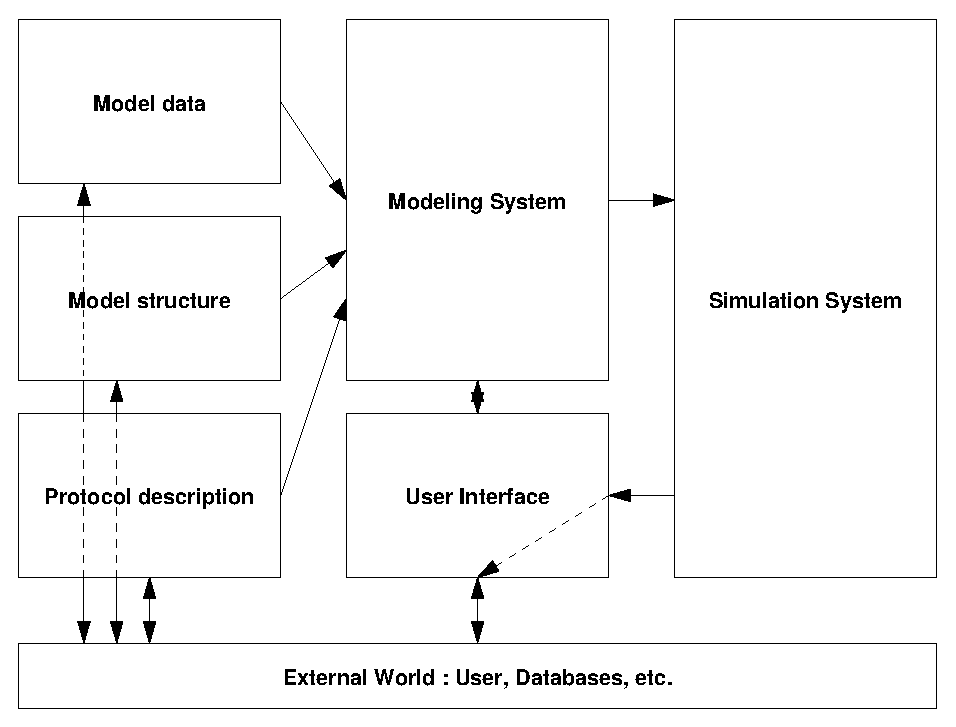
\includegraphics[scale=0.7]{figures/design.eps}
  \caption[Context of Neurospaces]
  {\small Context of NeuroSpaces\:: At the left are descriptions of
    the system to be simulated\:: the model data and structure and the
    experimental protocol if applicable.  All these descriptions could
    come from a database.  At the right is the simulation engine,
    which is the computational core of the whole system.  In the
    center, a software component that only supports the setup and
    validation of modeling.  During model construction, the user
    interacts with the modeling system.  During the simulation, all
    results are handed to the user via the user interface, such that
    the complexity of the simulation system remains hidden.  }
  \label{fig:neurospaces-context}
\end{figure}


\section{Design Overview}
\label{sec:neurospaces-design-overview}
The model-container can be run a stand-alone application, or can be
builtin in a simulator of choice.  Here we describe the features of
the model-container and its interface with the GENESIS-3 simulator.
This allows to simulate with GENESIS-3 the models that have been
constructed with the model-container.

The model-container consists of collaborating software components.
The implementation in C uses techniques like nested \texttt{struct}s
and pointers to function tables to allow extension of its core in
classical object-oriented programming
style\cite{sessions92:_class_const_c_c}\cite[Chapter
1]{stevens95:_tcp_ip_illus_volum}\cite{wiley90:_advan_c_progr}.
Specification of the supported objects and the relationships between
them is done with YAML data structures which are parsed with perl
scripts to produce the object-oriented class hierchies.  The scripts
employs instrumentation and aspect-orientation to facilite extension
with a couple of lines of YAML configuration.

These techniques reduce the code size to about
3.2MB\marginpar{update}, including realistic test cases and extensive
inline documentation.

Based on Bird numbers and Dataguides for semi-structure
data\cite{DBLP:conf/xsym/WeigelSM05, goldman97dataguides,
  goldman99approximate}, the functional core of the model-container is
the implementation of a graph data structure that efficiently
represents and stores repititive data with small variations in
structure or quantity parameters:
\begin{enumerate}
\item The nodes in the graph represent biological components,
  (components for short) and sometimes they are implicitly associated
  with a mathematical formula.  This is explained further in
  section~\ref{sec:neurospaces-defin-biol-comp}.  The nodes contain
  labels that identify the biological components.
%  Further every node
%  can act as a treespace node or a forestspace node.
\item Links between the nodes represent one of the following three
  properties:
  \begin{itemize}
  \item The nodes are connected in a hierarchical parent-child
    relationship.  For instance a dendritic segment can be the parent
    of a transmembrane current.
  \item The nodes are connected via a direct axonal connection.
    Computationally this may mean that a spike of the first neuron is
    translated to a discrete event before it reaches the synapse of
    the second neuron.
  \item The nodes are connected because they have a parameter in
    common.  For instance the membrane potential of a dendritic
    segment is a parameter of the segment (the parent) and of the
    transmembrane current (the child) (see below,
    section~\ref{sec:neurospaces-shared-variables}).
  \end{itemize}
%\item The implementation supports the use of multiple roots as
%  discussed in section~\ref{sec:treespace-final-discussion},
%  page~\pageref{sec:treespace-final-discussion}.
%  Section~\ref{sec:neurospaces-impl-forestsp} explains the use of
%  multiple roots in more detail.  
\item The code contains various consistency checks as discussed in
  section~\ref{sec:treespaces-consistency-checking}
  (page~\pageref{sec:treespaces-consistency-checking}).
%\item Memory efficiency measure\marginpar{Complete}.
\end{enumerate}

Because of the node labels, the forestspace acts as a symbol table.
It can be inspected via a small command-driven query engine, which is
called the querymachine.  The purpose of the querymachine is to debug
Neurospaces.  It supports completion on command names and node labels
(via the GNU readline library), but does not allow sophisticated
queries via logical connectives or aggregates.  Since the symbol table
contains a mapped treespace, it can be addressed in a hierarchical
way\:: the node labels separated with a '\texttt{/}' relate them via a
parent-child relationship.  '\texttt{..}' and '\texttt{\^}' are
pointers to the parent symbol while '\texttt{.}' is a pointer to the
current symbol.  '\texttt{->}' selects a field of the current symbol
(a field is a variable or a parameter, see below).  The process of
following a chain of hierarchical relationships is called
\emph{redirection}.  For example, if the current symbol is
\texttt{Ca\_pool}, the redirection of \texttt{.}  gives simply
\texttt{Ca\_pool}.

The complete software design overview is depicted in figure
\ref{fig:neurospaces-overview}.  To the left is a specification of the
model in a serialized form.  Currently only files are supported, but
the files have a purely declarative nature such that they can be
stored in a database.  A lexical analyzer transforms the file to a
stream of tokens that is parsed by a syntax analyzer.  The syntax
analyzer communicates the semantics of the data stream to Neurospaces
using a set of system calls.  The last biological component in the
data stream that has not fully been specified yet, is called the
active symbol.  Algorithmic specifications of, or changes to a
component are specified with tokens that reference the modules by name
(see section~\ref{sec:neurospaces-loadable-modules} and
section~\ref{sec:neurospaces-module-instances}).  The modules are
activated by the parser and interact with Neurospaces via the system
calls to get a reference to the active symbol.  The resulting token
stream goes into Neurospaces and behaves as a declarative mathematical
specification of the model to be simulated.  The system calls in
Neurospaces allow further validation or graphical output of (parts of)
the model and at the same time allow solvers\footnote{'Solvers' should
  be interpreted in a broad sense here, i.e. a solver is anything that
  communicates with Neurospaces to inspect a model.  So for
  Neurospaces a graphical user interface is just a solver.} to inspect
what they have to compute.  The numbering scheme of the forestspace is
used to find computed variables and to set up communication between
the solver instances.  Because the (forestspace) links are always in
the discrete event domain, the communication between solvers is
currently restricted to discrete events only.

\begin{figure}[p]
  \center
  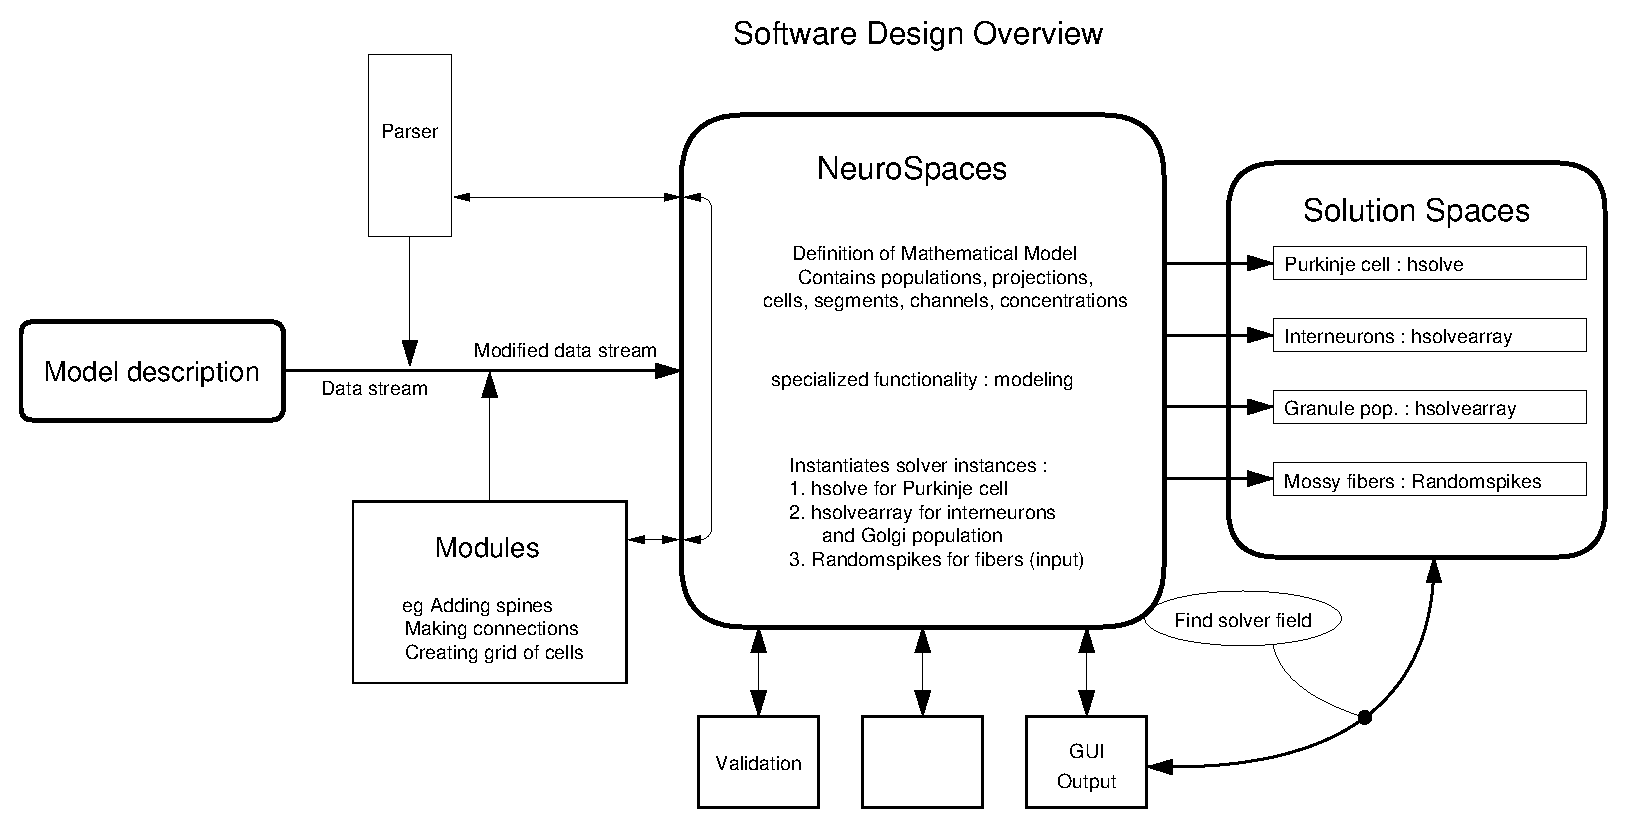
\includegraphics[angle=90,scale=0.75]{figures/model2.eps}
  \caption[Software Design Overview]
  {\small Software Design Overview of NeuroSpaces}
  \label{fig:neurospaces-overview}
\end{figure}
\afterpage{\clearpage}

In the next sections we discuss the different components in more
detail.

\section{Description files}
\label{sec:neurospaces-description-files}
In this section we discuss the philosophy behind the description files
with examples.  A single description file can contain one model or a
library of models.  To support modular construction of models, a
description file can depend on other description files.

The lexical analyzer first strips off any white-space and comments of
the following form\::
\begin{enumerate}
\item Normal C comments of the form \texttt{/* \ldots */}.  ~C comments may
  not be nested.
\item Normal C++ comments, starting with \texttt{//} and newline
  terminated.
\item Comments enclosed with \texttt{\{*} and \texttt{*\}}.  These
  comments may be nested.
\end{enumerate}

Afterwards the lexical analyzer transforms the remains of the
description file to a series of tokens.  Most lexical tokens have a
positive and a negative form.  If a positive is encountered, it must
be matched with a following negative.  It is forbidden to cross
couples of positive and negative tokens.  The nesting of positives and
negatives gives rise to a hierarchy.  This design is very close to
XML\cite{marsh01:_xml_base}.  Currently a perl script is used to
convert a description file to XML, and XSLT is used to convert the
resulting XML file back to a description
file\cite{clark01:_xsl_trans_xslt_version,
  muench01:_xslt_requir_version}.  However there is a possibility of
loss of information during the conversion with the perl script.

In the context of XML technologies, there has been a great interest in
the mapping of a declarative hierarchical file to a hierarchy of
run-time objects.  General examples of such technologies are
DOM\cite{group02:_docum_objec_model_dom}, JDOM\cite{hunter02:_jdom}
and even JavaScript\cite{flanagan:2002:jdg}.  Neuroscience oriented
examples are the NeuroML toolkit\cite{nigel01:_towar_neurom,
  howell02:_neurom_devel_kit} which had its origins in the work of
Michael Hucka from the Modelers Workspace
project\cite{hucka00:_prelim_defin_repres_schem_used_works} (now
updated by\cite{hucka00:_schuc}).  The fundamental principle of these
technologies is a one-to-one mapping of the hierarchy in the
declarative file to a hierarchy of run-time objects.  There are
several advantages as well as draw-backs to this method.  First the
method is simple, so it is straightforward to implement.  Second, the
run-time type of an object does not always need to be known (the
NeuroML toolkit uses dynamic lookup on Java class names to instantiate
the run-time objects).  The first major restriction however, is the
memory usage\:: all the run-time objects must be instantiated before
they can be handled by the client application.  The second major
restriction is that the mapping must be one-to-one.  Both of these
restrictions impose serious limitations on the software.  That is why
I first decided to analyze the nature of the lexical tokens in my
description files, before doing an implementation.

The lexical tokens fall in different categories\::
\begin{enumerate}
\item Some tokens define sections in a desription file.  The most
  important ones in this category are \texttt{IMPORT},
  \texttt{PRIVATE\_MODELS} and \texttt{PUBLIC\_MODELS}.  Models
  defined in one section can be forwarded to the next section with the
  \texttt{ALIAS} token.
\item Many tokens have the semantics of a specific physical process as
  defined in section~\ref{sec:state-space-abstr-real-world} on
  page~\pageref{sec:state-space-abstr-real-world}.  Examples are
  \texttt{EXP2\_EQUATION} for a dual exponential equation,
  \texttt{CHANNEL} for a Hodgkin-Huxley like conductance and
  \texttt{SEGMENT} for a cylindrical cable equation.  All these tokens
  map to a run-time C \texttt{struct}.  This \texttt{struct} is
  derived from one common structure to have inheritance of the
  capability of grouping (children) and having parameters.  A special
  case is the token \texttt{GROUP} that has no specific semantics
  except for the capability of grouping and having parameters.
\item Some tokens have the semantics of a function.  This is a special
  case of the above.  Examples are \texttt{randomize} to randomize a
  value and \texttt{FIXED} to calculate a constant value that cannot
  be scaled.  A special case is \texttt{SERIAL} that returns the
  (treespace) $\PrincipalSerial$ of the current symbol.
\item Other tokens exist to define the structure of a model\:: the
  \texttt{CHILD} token adds a new (reference to a) child to the active
  symbol.  The \texttt{PARAMETERS} token defines attributes on symbols
  with (name,value) tuples.  The \texttt{BINDABLES} allows to bind
  shared variables between different components.
\end{enumerate}

The models declared in a description file can be private to the
description file or public.  If a first file is dependent on a second
file, only the public models of the second file can be reused to build
more complicated models in the first file.  This mechanism allows to
protect access to certain declared components, while still allowing
reuse of other components.  The control on the access is private to
the description file.  This is important for incomplete models\::
parts of a model that are based on good experimental data, should be
constructed as public models.  However, if a lacking model of a
biological component is filled in, purely based on guess work and
intuition, the lacking piece should be constructed as a private model
to protect it from access by the outside world.  The fact that the
access control is centralized in a single file, facilitates model
maintenance.


\subsection{Sections in a Description File}

Any description file is a sequence of four sections, some possibly
empty (see figure~\ref{fig:neurospaces-description-sections})\::
\begin{enumerate}
\item The header always starts with the interpreter
  sequence\cite[Section 8.11]{stevens93:_advan_progr_unix_envir} \\
  \texttt{\#!neurospacesparse} \\
  After that comes a declaration to identify the type of file (i.e. a
  Neurospaces description file).  Other pieces, like declarations of
  the physical units used, are currently place-holders only.  They may
  be removed in a future version of the software.  The header must be
  present.
\item The import section declares dependencies on other description
  files with the \texttt{FILE} keyword.  To avoid naming conflicts,
  the public models in these files are attached to a namespace.  The
  namespace is alive during the import section and the private model
  section.  Afterwards it is discarded.
\item The private model section declares models private to the current
  file.  The models may depend on public models of imported files or
  be hardcoded.
\item The public model section declares models that are world visible.
  The models depend on private models or can be hardcoded.
\end{enumerate}

\begin{figure}[htbp]
  \centering
  \begin{boxedminipage}{10cm}
\begin{verbatim}
#!neurospacesparse
// -*- NEUROSPACES -*-
NEUROSPACES 0.2 NDF
VERSION 0.1
UNITS seconds meters voltage siemens
IMPORT
  FILE mapper "mappers/spikereceiver.ndf" 0.1
END IMPORT
PRIVATE_MODELS
  . . .
END PRIVATE_MODELS
PUBLIC_MODELS
  . . .
END PUBLIC_MODELS
\end{verbatim}
  \end{boxedminipage}
  \caption[The Sections in a Description File.]
  {\small The sections in a description file.}
  \label{fig:neurospaces-description-sections}
\end{figure}


\subsection{Definition of Models}

A model is a hierarchy of symbols, each representing a biological
component.  Each component is a physical process and can have
parameters and shared variables.  A parameter or a shared variable is
a field of the component.  Parameters are considered private to a
component, while shared variables have the intent to share their value
with other components as defined in
section~\ref{sec:state-space-abstr-real-world} on
page~\pageref{sec:state-space-abstr-real-world}.  This is the reason
that shared variables must be declared in the specification of the
model.  Parameters do not need to be declared.


\subsubsection{Parameter Specifications}
\label{sec:neurospaces-param-spec}
Parameters are (name,value) tuples.  Names are simple labels.  Values
can be specified as being constant, having the same value as a
parameter of another symbol or having a function value
(figure~\ref{fig:neurospaces-description-parameters}).  Parameters are
always specified within a \texttt{PARAMETERS} positive-negative block.
The parameter handling of Neurospaces is one of the most sophisticated
parts of the implementation.  Its complexity deals with a variety of
parameter types whereas its flexibility allows completely new
extensions to be implemented in a modular
way\cite{cornelis04:_neuros_param_handl}.  Some examples of the
parameter handling are given in
section~\ref{sec:neurospaces-querymachine}.

\begin{figure}[htbp]
  \centering
  \begin{boxedminipage}{7.5cm}
\begin{verbatim}
PARAMETERS
    PARAMETER ( DIAMETER =  0.3 ),
    PARAMETER ( LENGTH =  ^->LENGTH )
    PARAMETER ( SEED =  SERIAL() )
END PARAMETERS
\end{verbatim}
  \end{boxedminipage}
  \caption[Examples of Parameter Specifications.]
  {\small Examples of parameter specifications.  The \texttt{DIAMETER}
    parameter has a constant value, the \texttt{LENGTH} parameter is
    inherited from the parent component (the '\texttt{\^}' symbol is a
    reference to the parent symbol), the \texttt{SEED} parameter has
    the value of the mapped treespace $\PrincipalSerial$ of the active
    symbol.  Implicit is the coordinate of the component\:: it
    defaults to $(0,0,0)$.}
  \label{fig:neurospaces-description-parameters}
\end{figure}

Neurospaces allows to associate functions with a parameter, a feature
also supported by the parser.  A function can again have parameters.
Table~\ref{tab:neurospaces-functions} summarizes the most important
functions that are known by the parser and Neurospaces.  See
figure~\ref{fig:neurospaces-description-channel-use} for an example of
how to use the functions to specify parameter values.

\begin{table}
  \centering
  % token, math, bio, position aware.
  \begin{tabular}{|c|c|c|}
    \hline

    \rule[-3ex]{0mm}{7ex}
    Lexical Token & Mathematical Meaning & Biological Meaning \\

    \hline
    \hline

    \texttt{MGBLOCK}
    & $\frac{\exp(\frac{-t}{\tau_1}) - \exp(\frac{-t}{\tau_2})}{1
      + \eta[\mathrm{Mg}^{2+}] \cdot \exp(-\gamma V)}$
    & Magnesium blocking of a (NMDA) channel.
    \rule[-2ex]{0mm}{5ex}
    \\

%    \hline

    \texttt{NERNST}
    & $\frac{(T + 273.15)\mathrm{R}}{\mathrm{z}\mathrm{F}}
    \ln(\frac{[C]_{\mathrm{out}}}{[C]_{\mathrm{in}}})$
    & Nernst reversal potential.
    \rule[-2ex]{0mm}{5ex}
    \\

    \hline

    \texttt{SERIAL}
    & \multicolumn{2}{c|}{$\PrincipalSerial$, Makes all symbols unique.\rule[-2ex]{0mm}{5ex}}
    \\

%    \hline

%    & \multicolumn{2}{c|}{A random value between a minimum and a maximum.\rule[-2ex]{0mm}{5ex}}
    \texttt{STEP}
%    & $a \in [\mathrm{b},\mathrm{c}] $ \texttt{?} $1 : 0 \, ;$
%    & $1$ if $a$ between $\mathrm{b}$ and $\mathrm{c}$, otherwise $0$.
    & \multicolumn{2}{c|}{$1$ between two given values, otherwise $0$.\rule[-2ex]{0mm}{5ex}}
    \\

%    \hline

    \texttt{FIXED}
    & \multicolumn{2}{c|}{A fixed unscaled value.\rule[-2ex]{0mm}{5ex}}
    \\

%    \hline

    \texttt{randomize}
    & \multicolumn{2}{c|}{Uniform randomization between two boundaries.\rule[-2ex]{0mm}{5ex}}
    \\

%    \hline

    \hline

  \end{tabular}
  \caption
  [Neurospaces Functions]
  {\small Some of the component tokens known by
    the Neurospaces parser.  The mathematical entries give an approximate
    idea of the mathematical semantics.  For each element the biological
    meaning is given.
  }
  \label{tab:neurospaces-functions}
\end{table}


\subsubsection{Shared Variables}
\label{sec:neurospaces-shared-variables}
Shared variables must be declared together with the component that
they are attached to.  Declaration of shared variable is done with the
tokens \texttt{INPUT} and \texttt{OUTPUT} within a block of a
\texttt{BINDABLES} positive and negative.  Shared variables of one
component can be bound to shared variables of an other component.
Binding of shared variables corresponds to the binding as explained in
section~\ref{sec:state-space-abstr-real-world} on
page~\pageref{sec:state-space-abstr-real-world}.  The binding of
variables is done with \texttt{INPUT} tokens within a block of a
\texttt{BINDINGS} positive and negative.
Figure~\ref{fig:neurospaces-description-variables} gives an example of
shared variables specification and the binding of shared variables.

In the current implementation of Neurospaces, no \index{consistency
  checking}consistency checking is done on the shared variable
binding.

\begin{figure}[htbp]
  \centering
  \begin{boxedminipage}{9.1cm}
\begin{verbatim}
GROUP CalciumConductance
  BINDABLES
    INPUT Vm, OUTPUT CaHVA->Gk, OUTPUT CaHVA->Ik
  END BINDABLES
  CHILD Ca_concen Ca_pool
    BINDINGS
      INPUT CaHVA->Ik
    END BINDINGS
  END CHILD
  CHILD CaHVA CaHVA
    BINDINGS
      INPUT ^->Vm, INPUT ^/Ca_pool->concen
    END BINDINGS
  END CHILD
END GROUP
\end{verbatim}
  \end{boxedminipage}
  \caption[Example of shared variable specifications.]
  {\small Example of shared variable specifications.
    \texttt{CalciumConductance} is a group with two components\:: (1)
    an exponential decaying calcium pool \texttt{Ca\_pool} and (2) the
    channel \texttt{CaHVA} that is $\mathrm{Ca}^{2+}$ dependent (as
    indicated with the second input to the component).  The group has
    an input with label \texttt{Vm} and outputs with labels
    \texttt{Gk} and \texttt{Ik}.  The outputs are forwarded from the
    \texttt{CaHVA} channel.  A definition of a model comes always with
    a \texttt{BINDABLES} specification, while use of a model with the
    \texttt{CHILD} token comes always with a \texttt{BINDINGS}
    specification.  }
  \label{fig:neurospaces-description-variables}
\end{figure}


\subsubsection{Definition of Biological Components}
\label{sec:neurospaces-defin-biol-comp}
Tokens have been assigned to the most common neuro-biological
components.  Table~\ref{tab:neurospaces-components} gives an idea
about the components supported by Neurospaces\footnote{The kinetics of
  a \textrm{CHANNEL} component must be specified with a legacy Genesis
  table file.  At the moment of writing Genesis must be used to create
  these files.}.  Figure~\ref{fig:neurospaces-description-channel} is
an example of a definition of a channel model.  The use of the channel
is shown in figure~\ref{fig:neurospaces-description-channel-use}.  The
examples are straightforward, and show many of the possibilities of
the description format.


\begin{table}
  \centering
  % token, math, bio, position aware.
  \begin{tabular}{|c|c|c|}
    \hline

    \rule[-3ex]{0mm}{7ex}
    Lexical Token & Mathematical Meaning & Biological Meaning \\

    \hline
    \hline

    \texttt{EXP2\_EQUATION}
    & $ \frac{\mathrm{d}^2G}{(\mathrm{d}t)^2}
    + \alpha \frac{\mathrm{d}G}{\mathrm{d}t} + \beta G = \sum_i \delta(t - t_i) $
    & Synaptic channel.
    \rule[-2ex]{0mm}{5ex}
    \\

%    \hline

    \texttt{POOL}
    & $ D = D_{base} + C, \; \frac{\mathrm{d}C}{\mathrm{d}t}
    = \mathrm{B} \cdot \mathrm{I} - \frac{C}{\tau} $
    & Simple ion concentration
    \rule[-2ex]{0mm}{5ex}
    \\

%%    \hline

    \texttt{CHANNEL}
    & $ G = \overline{\mathrm{g}} x^\mathrm{X} y^\mathrm{Y} z^\mathrm{Z} $
    or $G$ for synchannels.
    & Hodgkin-Huxley or synchannel.
    \rule[-2ex]{0mm}{5ex}
    \\

%    \hline

    \texttt{SEGMENT}
    & $   \frac{a}{2R_a}\frac{\partial^2V}{\partial x^2} = C_m \frac{\partial V}{\partial t} +
    I_{\mathrm{HH}} $
    & A cylindrical dendritic segment.
    \rule[-2ex]{0mm}{5ex}
    \\

%    \hline

    \texttt{SPIKEGEN}
    & Attachment point for outgoing links.
    & Starting point of the axon.
    \rule[-2ex]{0mm}{5ex}
    \\

%    \hline

    \texttt{SYNAPSE}
    & Attachment point for incoming links.
    & Possibility to have a synapse.
    \rule[-2ex]{0mm}{5ex}
    \\

    \hline

    \texttt{RANDOMVALUE}
    & \multicolumn{2}{c|}{A random value between a minimum and a maximum.\rule[-2ex]{0mm}{5ex}}
    \\

%    \hline

    \texttt{SEGMENT\_GROUP}
    & \multicolumn{2}{c|}{Enumeration of segments.\rule[-2ex]{0mm}{5ex}}
    \\

%    \hline

    \texttt{CELL}
    & \multicolumn{2}{c|}{A neuron with a dendrite.\rule[-2ex]{0mm}{5ex}}
    \\

%    \hline

    \texttt{POPULATION}
    & \multicolumn{2}{c|}{Enumeration of cells, a neuron population.\rule[-2ex]{0mm}{5ex}}
    \\

%    \hline

    \texttt{CONNECTION\_GROUP}
    & \multicolumn{2}{c|}{Enumeration of connections.\rule[-2ex]{0mm}{5ex}}
    \\

%    \hline

    \texttt{CONNECTION}
    & \multicolumn{2}{c|}{Connection between a spike generator and a \texttt{SYNAPSE}.\rule[-2ex]{0mm}{5ex}}
    \\

%    \hline

    \texttt{PROJECTION}
    & \multicolumn{2}{c|}{Enumeration of connection groups, a biological projection.\rule[-2ex]{0mm}{5ex}}
    \\

%    \hline

    \texttt{NETWORK}
    & \multicolumn{2}{c|}{Networks, populations and projections, a (biological) neural network.\rule[-2ex]{0mm}{5ex}}
    \\

    \hline

  \end{tabular}
  \caption
  [Neurospaces Component Lexical Tokens]
  {\small Some of the component tokens known by
    the Neurospaces parser.  The mathematical entries give an approximate
    idea of the mathematical semantics.  For all elements the biological
    meaning is given.
  }
  \label{tab:neurospaces-components}
\end{table}


\begin{figure}[htbp]
  \centering
  \begin{boxedminipage}{15cm}
\begin{verbatim}
#!neurospacesparse
// -*- NEUROSPACES -*-
NEUROSPACES 0.2 NDF VERSION 0.1 UNITS seconds meters voltage siemens
IMPORT FILE mapper "mappers/spikereceiver.ndf" 0.1 END IMPORT
PRIVATE_MODELS ALIAS mapper::/Synapse Synapse END ALIAS END PRIVATE_MODELS
PUBLIC_MODELS
  CHANNEL Purk_GABA
    BINDABLES INPUT Vm,OUTPUT exp2->Gk,OUTPUT Ik END BINDABLES
    PARAMETERS PARAMETER ( GMAX = 1.077 ),PARAMETER ( Ek = 0.0 ) END PARAMETERS
    CHILD Synapse synapse END CHILD
    EXP2_EQUATION exp2
      BINDABLES INPUT activation,OUTPUT Gk END BINDABLES
      BINDINGS INPUT ^/synapse->activation END BINDINGS
      PARAMETERS
        PARAMETER ( TAU1 = 0.93e-3 ),PARAMETER ( TAU2 = 26.50e-3 )
      END PARAMETERS
    END EXP2_EQUATION
  END CHANNEL
END PUBLIC_MODELS
\end{verbatim}
  \end{boxedminipage}
  \caption[Example of a Channel Model Specification.]
  {\small The specification of a synaptic channel model.  The channel
    contains a dual exponential equation that receives discrete events
    via the synapse and the \texttt{activation} input.  The activation
    is the driving force for a second order differential equation (see
    table~\ref{tab:neurospaces-components}).  The dual exponential
    component gives the conductance that is fed to the channel
    component.  The channel component has an input of a potential
    (\textrm{Vm}) that allows it to compute the current
    (\textrm{Ik}).}
  \label{fig:neurospaces-description-channel}
\end{figure}

\begin{figure}[htbp]
  \centering
  \begin{boxedminipage}{15cm}
\begin{verbatim}
#!neurospacesparse
// -*- NEUROSPACES -*-
NEUROSPACES 0.2 NDF VERSION 0.1 UNITS seconds meters voltage siemens
IMPORT
  FILE GABA "channels/gaba.ndf" 0.1
  FILE CaP "channels/purkinje_cap.ndf" 0.1
  FILE Ca_pool "pools/purkinje_ca.ndf" 0.1
END IMPORT
PRIVATE_MODELS
  ALIAS GABA::/Purk_GABA GABA END ALIAS
  ALIAS CaP::/CaP CaP END ALIAS
  ALIAS Ca_pool::/Ca_concen Ca_pool END ALIAS
END PRIVATE_MODELS
PUBLIC_MODELS
  SEGMENT Purk_thickd
    BINDABLES OUTPUT Vm END BINDABLES
    BINDINGS INPUT CaP->Ik,INPUT stellate1->Ik, END BINDINGS
    PARAMETERS
      PARAMETER ( Vm_init = -0.0680 ), PARAMETER ( RM = 3.0 ),
      PARAMETER ( RA = 2.50 ), PARAMETER ( CM = 0.0164 ),
      PARAMETER ( ELEAK = -0.0800 )
    END PARAMETERS
    CHILD Ca_pool Ca_pool BINDINGS INPUT ^/CaP->Ik END BINDINGS END CHILD
    CHILD CaP CaP BINDINGS INPUT ^->Vm END BINDINGS
      PARAMETERS
        PARAMETER ( GMAX = 45.0 ),
        PARAMETER ( Ek = NERNST
                    (PARAMETER ( Cin = ^/Ca_pool->concen ),
                     PARAMETER ( Cout = 2.4 ),
                     PARAMETER ( valency = ^/Ca_pool->VAL) ,/* 2.0, */
                     PARAMETER ( T = 37.0) ))
      END PARAMETERS
    END CHILD
    CHILD GABA stellate1
      BINDINGS INPUT ^->Vm END BINDINGS
      PARAMETERS
        PARAMETER ( GMAX = 14.0 ), PARAMETER ( Ek = -0.080 ),
        PARAMETER ( FREQUENCY = 0.0 )
      END PARAMETERS
    END CHILD
  END SEGMENT
END PUBLIC_MODELS
\end{verbatim}
  \end{boxedminipage}
  \caption[Example of Channel Model Use.]
  {\small An example how to use the previously defined channel (see
    figure~\ref{fig:neurospaces-description-channel}).  The file
    containing the channel is imported (\texttt{gaba.ndf}) and a
    namespace (\texttt{GABA}) is associated with it.  Also some other
    files are imported.  In the private model section, the models in
    the namespaces that must be part of the model to be built, are
    aliased to make them accessible in the public model section.
    Next, the channel (label \texttt{stellate1}) is used in a cable
    segment (label \texttt{Purk\_thickd}).  The segment also contains a
    calcium pool and a calcium channel.  Note that the reversal
    potential of the calcium channel is specified to be dependent on
    the nernst function.  The parameters of the function are again
    dependent on the calcium concentration.  Although incomplete from
    a biological viewpoint, this model is a good example of the
    complexity supported by the model description format.}
  \label{fig:neurospaces-description-channel-use}
\end{figure}


%\begin{verbatim}
%#!neurospacesparse
%// -*- NEUROSPACES -*-
%NEUROSPACES 0.2 NDF VERSION 0.1 UNITS seconds meters voltage siemens
%IMPORT
%  FILE GABA "channels/gaba.ndf" 0.1
%  FILE non_NMDA "channels/non_nmda.ndf" 0.1
%  FILE CaP "channels/purkinje_cap.ndf" 0.1
%  FILE CaT "channels/purkinje_cat.ndf" 0.1
%  FILE K2 "channels/purkinje_k2.ndf" 0.1
%  FILE KA "channels/purkinje_ka.ndf" 0.1
%  FILE KC "channels/purkinje_kc.ndf" 0.1
%  FILE Kdr "channels/purkinje_kdr.ndf" 0.1
%  FILE KM "channels/purkinje_km.ndf" 0.1
%  FILE Ca_pool "pools/purkinje_ca.ndf" 0.1
%END IMPORT
%PRIVATE_MODELS
%  ALIAS GABA::/Purk_GABA GABA END ALIAS
%  ALIAS non_NMDA::/Purk_non_NMDA non_NMDA END ALIAS
%  ALIAS CaP::/CaP CaP END ALIAS
%  ALIAS CaT::/CaT CaT END ALIAS
%  ALIAS K2::/K2 K2 END ALIAS
%  ALIAS KA::/KA KA END ALIAS
%  ALIAS KC::/KC KC END ALIAS
%  ALIAS Kdr::/Kdr Kdr END ALIAS
%  ALIAS KM::/KM KM END ALIAS
%  ALIAS Ca_pool::/Ca_concen Ca_pool END ALIAS
%END PRIVATE_MODELS
%PUBLIC_MODELS

%  // normal definition for segments of a thick dendrite of a
%  // Purkinje cell

%  SEGMENT Purk_thickd
%    BINDABLES OUTPUT Vm END BINDABLES
%    BINDINGS
%      INPUT CaP->Ik,
%      INPUT CaT->Ik,
%      INPUT K2->Ik,
%      INPUT KC->Ik,
%      INPUT KM->Ik,
%      INPUT stellate1->Ik,
%      INPUT stellate2->Ik,
%      INPUT climb->Ik
%    END BINDINGS
%    PARAMETERS
%      PARAMETER ( Vm_init = -0.0680 ),
%      PARAMETER ( RM = 3.0 ),
%      PARAMETER ( RA = 2.50 ),
%      PARAMETER ( CM = 0.0164 ),
%      PARAMETER ( ELEAK = -0.0800 )
%    END PARAMETERS

%    // = calcium related things

%    CHILD Ca_pool Ca_pool
%      BINDINGS INPUT ^/CaT->Ik,INPUT ^/CaP->Ik END BINDINGS
%    END CHILD
%    CHILD CaT CaT
%      BINDINGS INPUT ^->Vm END BINDINGS
%      PARAMETERS
%        PARAMETER ( GMAX = 5.0 ),
%        PARAMETER
%        ( Ek = NERNST
%          (PARAMETER ( Cin = ^/Ca_pool->concen ),
%            PARAMETER ( Cout = 2.4 ),
%            PARAMETER ( valency = ^/Ca_pool->VAL) ,/* 2.0, */
%            PARAMETER ( T = 37.0) ))
%      END PARAMETERS
%    END CHILD
%    CHILD CaP CaP
%      BINDINGS INPUT ^->Vm END BINDINGS
%      PARAMETERS
%        PARAMETER ( GMAX = 45.0 ),
%        PARAMETER
%        ( Ek = NERNST
%          (PARAMETER ( Cin = ^/Ca_pool->concen ),
%            PARAMETER ( Cout = 2.4 ),
%            PARAMETER ( valency = ^/Ca_pool->VAL) ,/* 2.0, */
%            PARAMETER ( T = 37.0) ))
%      END PARAMETERS
%    END CHILD

%    // calcium dependent channels

%    CHILD KC KC
%      BINDINGS INPUT ^->Vm,INPUT ^/Ca_pool->concen END BINDINGS
%      PARAMETERS
%        PARAMETER ( GMAX = 800.0 ),
%        PARAMETER ( Ek = -0.085 )
%      END PARAMETERS
%    END CHILD

%    CHILD K2 K2
%      BINDINGS INPUT ^->Vm,INPUT ^/Ca_pool->concen END BINDINGS
%      PARAMETERS
%        PARAMETER ( GMAX = 3.90 ),
%        PARAMETER ( Ek = -0.085 )
%      END PARAMETERS
%    END CHILD

%    // active channels

%    CHILD KM KM
%      BINDINGS INPUT ^->Vm END BINDINGS
%      PARAMETERS
%        PARAMETER ( GMAX = 0.130 ),
%        PARAMETER ( Ek = -0.085 )
%      END PARAMETERS
%    END CHILD

%    // channels with synapses

%    CHILD GABA stellate1
%      BINDINGS INPUT ^->Vm END BINDINGS
%      PARAMETERS
%        PARAMETER ( GMAX = 14.0 ), // 70.0 / 5
%        PARAMETER ( Ek = -0.080 ),
%        PARAMETER ( FREQUENCY = 0.0 )
%      END PARAMETERS
%    END CHILD
%    CHILD GABA stellate2
%      BINDINGS INPUT ^->Vm END BINDINGS
%      PARAMETERS
%        PARAMETER ( GMAX = 14.0 ), // 70.0 / 5
%        PARAMETER ( Ek = -0.080 ),
%        PARAMETER ( FREQUENCY = 0.0 )
%      END PARAMETERS
%    END CHILD
%    CHILD non_NMDA climb
%      BINDINGS INPUT ^->Vm END BINDINGS
%      PARAMETERS
%        PARAMETER ( GMAX = 150.0 ),
%        PARAMETER ( Ek = 0.0 )
%      END PARAMETERS
%    END CHILD
%  END SEGMENT
%END PUBLIC_MODELS
%\end{verbatim}



\section{Internal Design}

As already noted, the core of Neurospaces is the implementation of a
labeled forestspace that acts as a \index{symbol table}symbol table.
Besides the forestspace, many collaborating software components can be
identified (see figure~\ref{fig:neurospaces-internals}).

\begin{figure}[htbp]
  \centering
  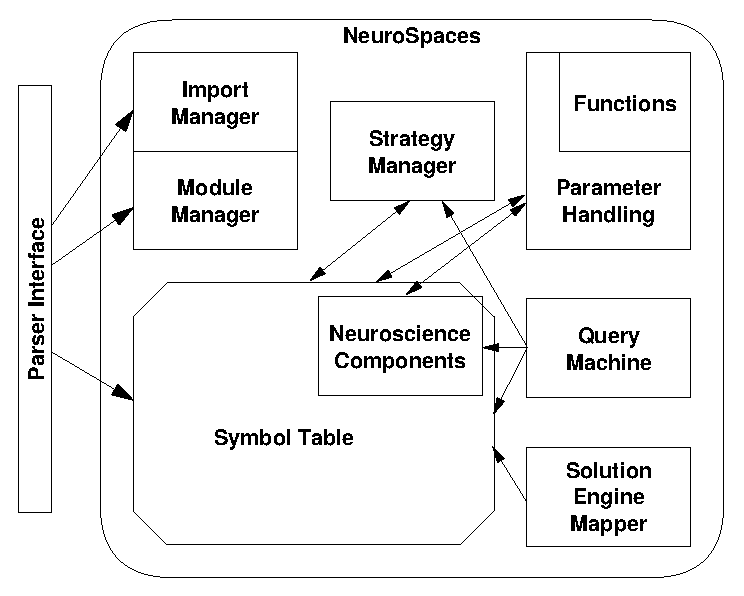
\includegraphics[scale=0.7]{figures/internal.eps}
  \caption[Neurospaces Internals]
  {\small The internal design of NeuroSpaces\:: The import manager
    lets the parser know which files to load.  The module manager
    interacts with the parser for the context of the activation of the
    modules.  The result of parsing a file is a \index{symbol
      table}symbol table that uses a forestspace to store the model in
    a compact form.  A special module for parameter handling
    implements scaling of conductances and relative coordinates.  The
    solution engine mapper allows to instantiate specialized solvers,
    specific for certain model structures.  It is a part of the
    configuration of a simulation schedule.  The strategy manager
    provides system calls to traverse parts of the forestspace.  The
    query machine allows to inspect the \index{symbol table}symbol
    table.  It is used for debugging only.}
  \label{fig:neurospaces-internals}
\end{figure}

\subsection{Implementation of the Forestspace}
\label{sec:neurospaces-impl-forestsp}
\subsubsection{Nodes and Components}

The \index{symbol table}symbol table containing all biological
components is implemented with a multiple indexed forestspace,
extended with multiple roots.  The structure of the forestspace can be
characterized as follows\::

\begin{enumerate}
\item The public and private model section of each description file is
  mapped to a root of a forestspace.
\item Each biological component, specified in a description file or
  created by a module, is mapped to a treespace node.
\item The \texttt{CHILD} and \texttt{ALIAS} tokens are mapped to
  reference nodes.  The referee of the child is responsible for
  creating a node that acts as an alias of the referee.  The reference
  node is bound to the forestspace with an \index{upper right
    union}upper right union, explained in
  section~\ref{sec:treespaces-constr-single-index}
  (page~\pageref{sec:treespaces-constr-single-index}), or a
  generalization thereof.
\item There is an implicit biological level associated with each
  component.  This is to ensure that a \texttt{CELL} does not contain
  a \texttt{NETWORK} for example.  Nevertheless currently no
  \index{consistency checking}consistency checking is done on this.
  It is the responsibility of the description file to specify a model
  that is well structured.
\end{enumerate}

Figure~\ref{fig:neurospaces-network-forest} gives an example
forestspace for a model of the granular layer of the cerebellar cortex
network and illustrates the sharing of biological components.


\begin{figure}[htbp]
  \centering
  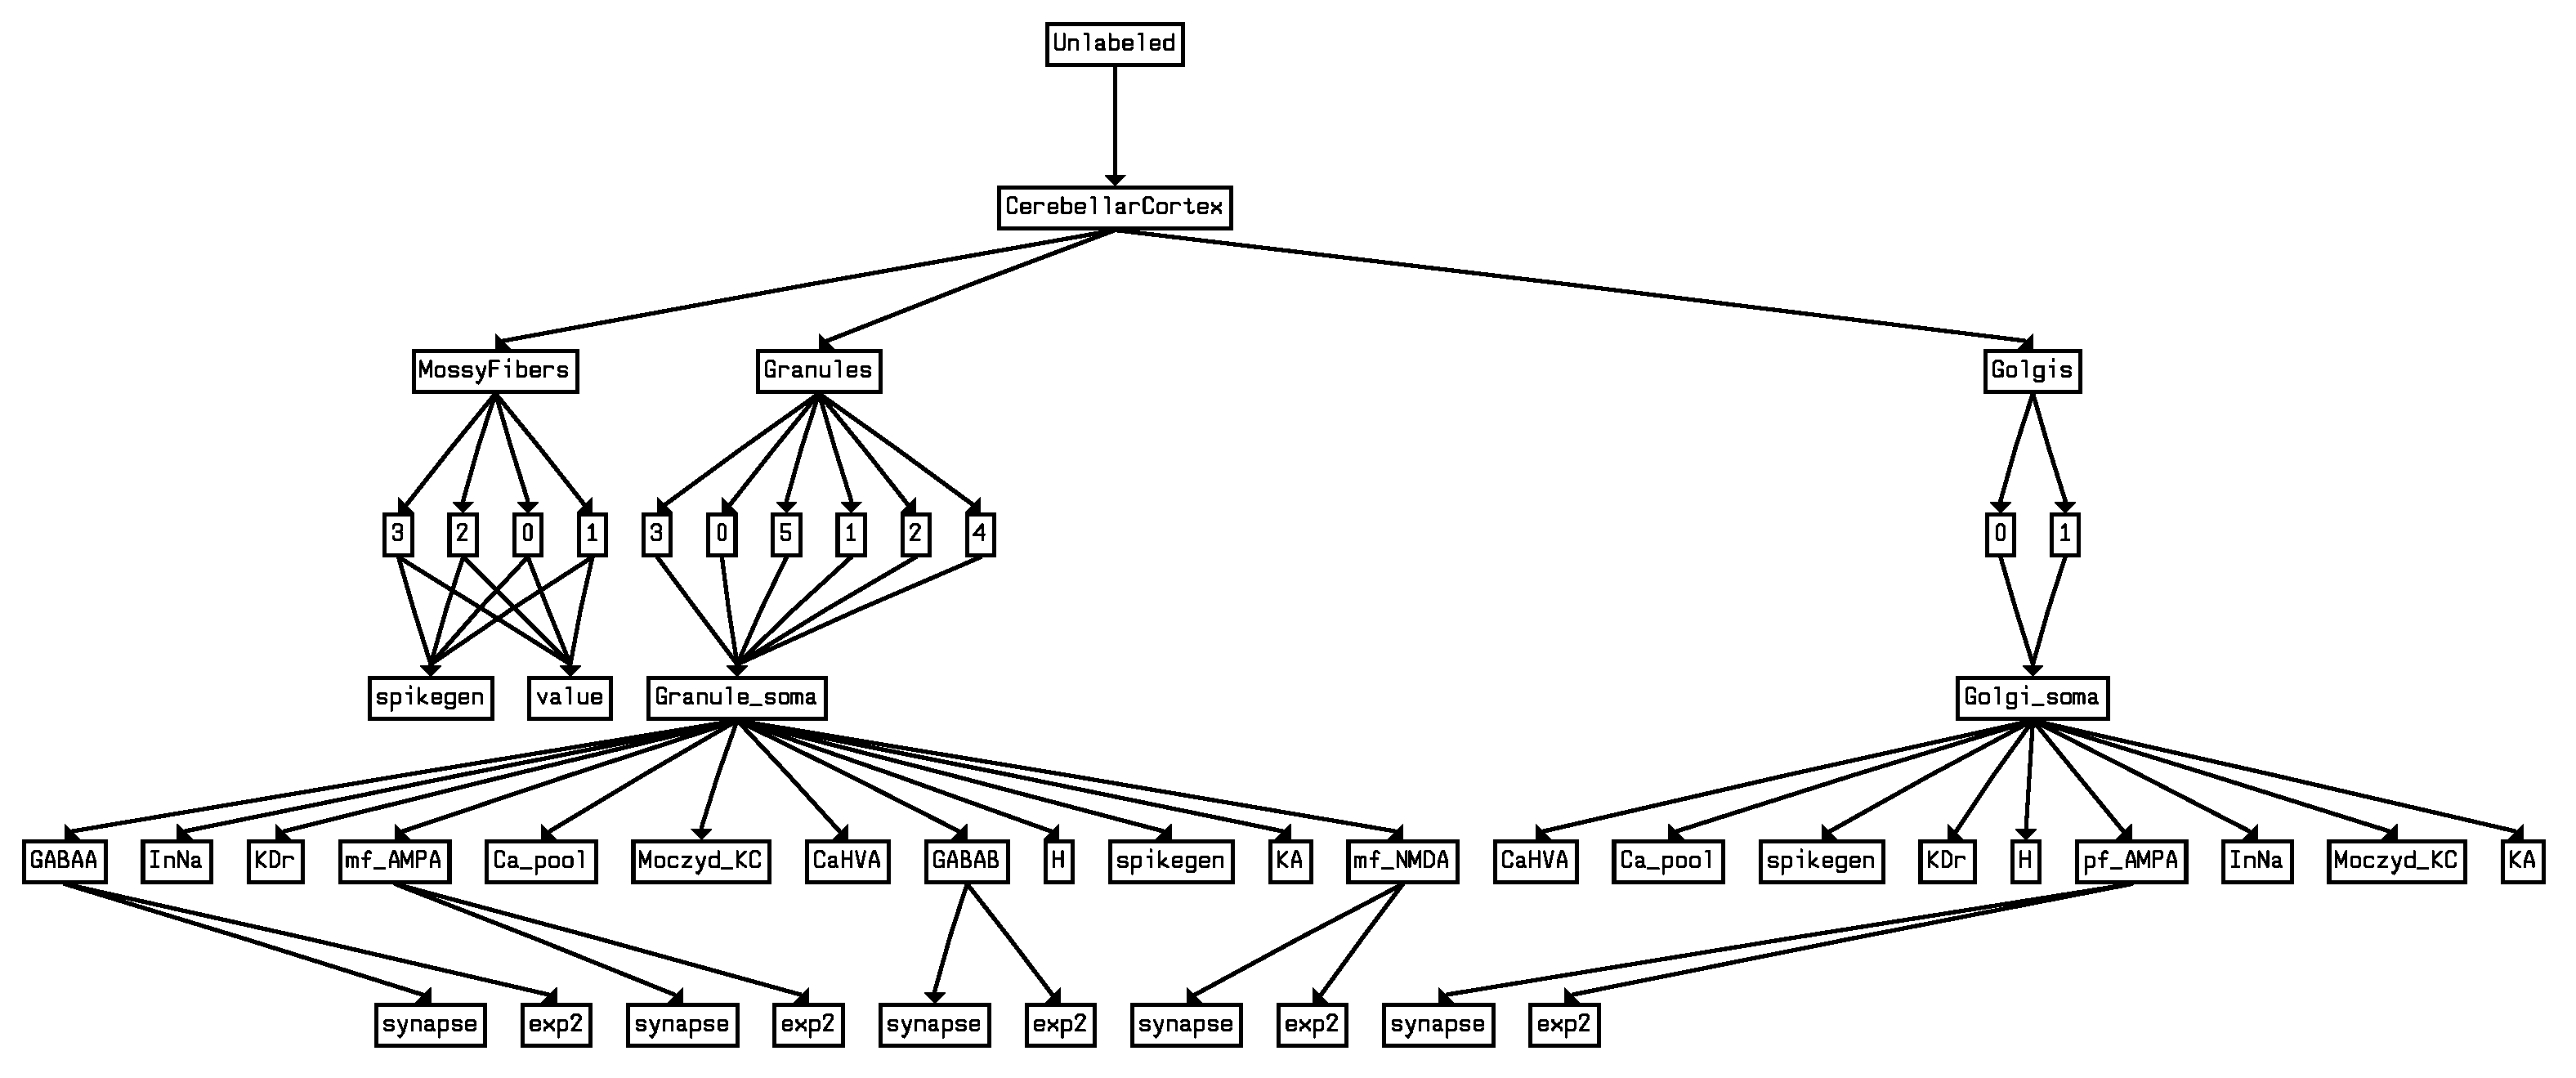
\includegraphics[scale=0.29]{figures/network-forest.eps}
  \caption[Forestspace Created for a Cerebellar Cortex Network.]
  {\small A part of the forestspace created for an instance of the
    cerebellar cortex network.  Only treespace nodes are shown, the
    reference nodes are implicit in the edges between the treespace
    nodes (if any).
    
    At the top is the public model section of the file.  The second
    level contains the network node.  The third level contains three
    populations\:: the mossy fiber population (4 fibers), the granule
    cell population (6 cells) and the Golgi cell population (2 cells).
    Below the cells or fibers comes a subgraph that describes their
    properties (morphology, channels, etc\ldots).  The nodes representing
    the projections and connections in the network are not shown.  }
  \label{fig:neurospaces-network-forest}
\end{figure}


At run-time, the biological components are represented in memory as C
\texttt{struct}s.  Nesting these structures and a disciplined
programming style gives the source code a feeling close to
object-oriented programming.  The derivation hierarchy is shown in
figure~\ref{fig:neurospaces-component-hierarchy}.

\begin{figure}[htbp]
  \centering
  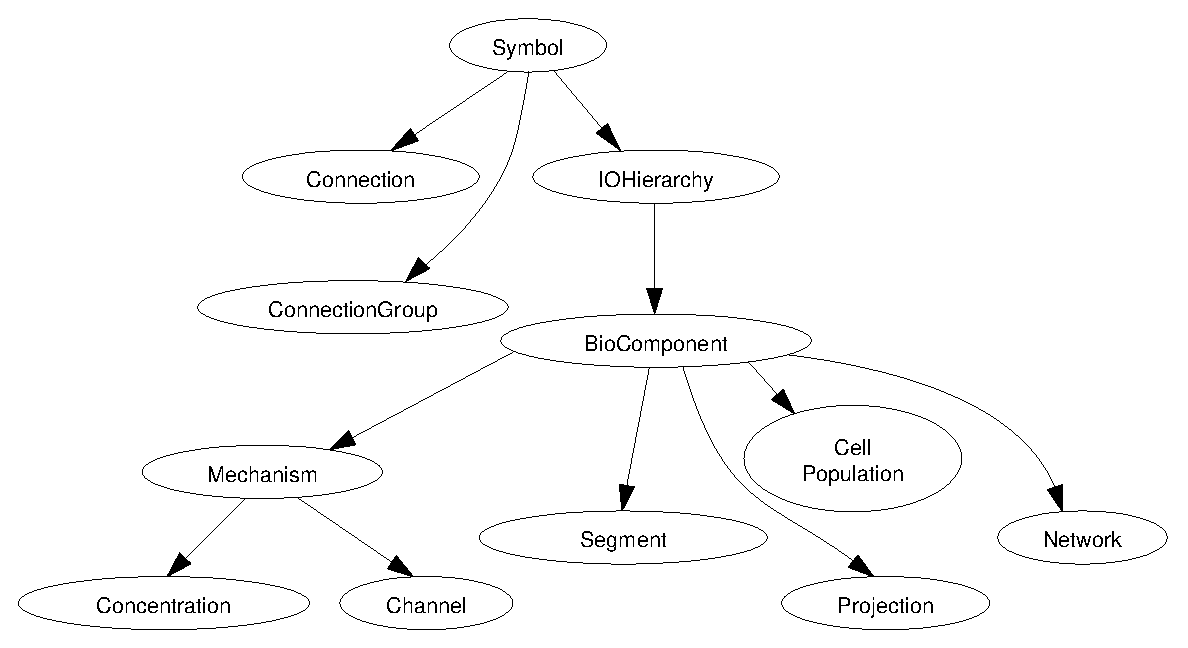
\includegraphics[scale=0.78]{figures/hier-poster.eps}
  \caption[Component Hierarchy]
  {\small Embedding C \texttt{struct}s gives rise to the shown type
    hierarchy for the biological components.  All biological
    components are derived from \texttt{Symbol} which implements
    treespace numbering.  \texttt{IOHierarchy} knows how to handle
    shared variables and parameters, the \texttt{BioComponent} gives
    capability of prototyping (reference nodes for a forestspace).
    The leaves represent types of models of biological components.}
  \label{fig:neurospaces-component-hierarchy}
\end{figure}


\subsubsection{\index{discrete event}Discrete Event Connections}

The communication between neurons in a model of a neural network
occurs via discrete event connections.  As already mentioned in the
introduction of this chapter (see
section~\ref{sec:neurospaces-design-overview}), the discrete event
connections are implemented with treespace links.  This allows the
attachment of different simulation processes to different sets of
neurons based on the theoretical framework described in
chapter~\ref{cha:state-space}.  The \index{treespace link}treespace
links that represent the discrete event connections, have two
attributes, \texttt{WEIGHT} and \texttt{DELAY}, that correspond to the
weight of a biological synapse and the delay of axonal signal
propagation.  This way of modeling axons and synapses is slightly
different from the way it is implemented by the most common
simulators\cite{bower98:_book_genes, hines97:_neuron_simul_envir,
  skrzypek94:_neural_networ_simul_envir,
  vilbert01:_xnbc_v9_simul_analy_tool_neurob}.  In Genesis, the weight
and delay of a connection is associated with the synapse (see
section~\ref{sec:example-gran-layer-netw}).

The attachment points in the \index{symbol table}symbol table of
Neurospaces model the transitions from the continuous time domain to
the discrete event domain and vice-versa.  The \texttt{SPIKEGEN}
element, an \index{output attachment point}output attachment point,
maps from the continuous time domain to the discrete event domain, the
\texttt{SYNAPSE} element, an \index{input attachment point}input
attachment point, the opposite way.  The presence of these elements
does not imply a connection, but the possibility to attach
connections.  The connections can then be created and associated with
a delay and a weight (normally the connections will be created by a
module, see section~\ref{sec:neurospaces-loadable-modules}).

A connection is modeled with a \texttt{CONNECTION} element.
Connections are unlabeled elements and are enumerated in a
\texttt{CONNECTION\_GROUP} element.  A set of \texttt{CONNECTION\_GROUP}
elements makes up a \texttt{PROJECTION} element, a biological
projection.  A projection is implemented with a treespace link at the
\index{population level}population and \index{network level}network
level, while a connection is a treespace link at the \index{mechanism
  level}mechanism level.


\subsection{Modules}
\label{sec:neurospaces-loadable-modules}

Modules in Neurospaces are intended to implement algorithmic
specifications of a model i.e. everything that does not fit a compact
declarative specification.  Examples of what modules can do are\::

\begin{enumerate}
\item Remove components from a model\:: remove cells from a
  population, remove segments from a cell,\ldots
\item Adjust parameters, e.g. the randomization of the \index{leak
    conductance}leak conductance of the segments in a population
  according to a probability distribution,\ldots
\item Create new components\:: add spines or synapse attachment points
  to small segments, add projections and connection groups to a
  network.
\item Do layout of components\:: calculate positions of cells in a
  network to put them in a grid.
\item Check if the model obeys known biological constraints.
\end{enumerate}

The implementation of a module is called the class of the module.  At
run-time, Neurospaces knows all module classes by name.  In a
description file, a reference to a module is made with the name of the
module class and parameters describing the action the module should
perform.  Neurospaces activates the code of the module with parameters
describing the context of the current symbol and the raw parameters
that have been given in the description file.  The module parses the
parameters and performs its actions to build a resulting model.
Neurospaces is notified of a description of the actions that the
module has taken and the resulting model is incorporated into the
\index{symbol table}symbol table.

This way the code of a module is a (type of) algorithm while the
reference to the module, made in the description file is an instance
of the algorithm.  Every instantiated module is given a name (in the
description file), which is kept by Neurospaces for later reference
(see also
figures~\ref{fig:neurospaces-description-modules-use-spines},
\ref{fig:neurospaces-description-modules-use-grid},
\ref{fig:neurospaces-description-modules-use-connections}
and~\ref{fig:neurospaces-module-instances}).


\section{Some Examples with the Querymachine}
\label{sec:neurospaces-querymachine}

The querymachine is a small and very simple query engine that allows
to inspect the \index{symbol table}symbol table.  Its primary purpose
is the debugging of Neurospaces.  The querymachine contains several
hardcoded constructions that quickly become obsolete for an evolving
research project.  Nevertheless it has proven very useful and I will
use it to demonstrate some of the topics discussed in the previous
sections.

If Neurospaces is run in stand-alone mode, the querymachine is invoked
with the \texttt{-q} option on the command line.  If Neurospaces is
run from Genesis, the action \texttt{NEUROSPACES\_QUERY} must be
invoked to enter the querymachine.  The querymachine behaves
identically in the two scenarios.

%%\begin{figure*}[htbp]
%%  \centering
%  \begin{boxedminipage}{13cm}
%\begin{verbatim}
%  genesis > call neurospaces NEUROSPACES_QUERY
%\end{verbatim}
%  \end{boxedminipage}
%%  \caption[Invoking the Querymachine]
%%  {\small Invoking the Querymachine.}
%%  \label{fig:neurospaces-invoking-querymachine}
%%\end{figure*}


\subsection{Inspecting Serial Identification Numbers}
\label{sec:neurospaces-insp-seri-ident}
Since we are dealing with the first ever implementation of a
forestspace, inspecting the serial identification numbers of the
biological components is an interesting exercise.  As proof of
concept, Neurospaces takes two subsets of the principal set (the set
of all components)\::
\begin{itemize}
\item All components of a type derived from \texttt{segment}
  (inclusive), belong to the segment subset.
\item All biological components that can be children of a
  \texttt{segment} or children of a component derived from a
  \texttt{segment} belong to the mechanism subset.  These are channels
  and concentrations, but not e.g.  \texttt{GROUP} (since it is not a
  biological component).
\end{itemize}

To inspect the serial identification numbers, the
\texttt{serialMapping} command is used with two arguments.  The first
argument ($a$) is the context (a context is a pathname that refers to
a symbol in the \index{symbol table}symbol table) of a component in
the \index{symbol table}symbol table, the second argument ($b$) is the
context of one of the descendants of the first component.  The command
first reports the expected identification number for $b$ relative to
$a$ by performing an explicit treespace traversal of the forestspace.
Then a report is given on the numbers $\PrincipalSerial_a(b)$ and
$\PrincipalDescendants(a)$, for each of the three (sub)sets.  This is
shown in figure~\ref{fig:neurospaces-serial-mapping}.

\begin{figure}[htbp]
  \centering
  \begin{boxedminipage}{13cm}
\begin{verbatim}
neurospaces > serialMapping / /CerebellarCortex/Granules
  Traversal serial ID = 93
  Principal serial ID = 93 of 214562 Principal successors
  Mechanism serial ID = 0 of 82844 Mechanism successors
  Segment  serial  ID = 0 of 27778  Segment  successors
neurospaces > serialMapping \
                /CerebellarCortex/Granules
                /CerebellarCortex/Granules/23/Granule_soma/spikegen
  Traversal serial ID = 509
  Principal serial ID = 509 of 10560 Principal successors
  Mechanism serial ID = 253 of 5280 Mechanism successors
  Segment  serial  ID = 24 of 480  Segment  successors
neurospaces > serialMapping / \
        /CerebellarCortex/Granules/23/Granule_soma/spikegen
  Traversal serial ID = 602
  Principal serial ID = 602 of 214562 Principal successors
  Mechanism serial ID = 253 of 82844 Mechanism successors
  Segment  serial  ID = 24 of 27778  Segment  successors
\end{verbatim}
  \end{boxedminipage}
  \caption[Serial Mapping in Neurospaces.]
  {\small Inspecting the serial mapping with the querymachine.  The
    first query reports the serial identification number for the
    granule cell population, the second query a component of the 23th
    cell of the granule population, but relative to the population
    component.  The third query inspects the identification number of
    the same component, but relative to the root.  Of course adding
    the two first numbers, gives the third number.  From the first
    query, one also learns that there are a total of 214562 components
    in this particular network model.  (Note\:: Neurospaces uses the
    word 'successors' instead of 'descendants'.) }
  \label{fig:neurospaces-serial-mapping}
\end{figure}

The \texttt{serial2context} command is the counterpart of the
\texttt{serialMapping} command.  It takes as arguments a context and
an identification number, and outputs the context referenced by the
identification number (see
section~\ref{sec:neurospaces-insp-netw-conn} for an example).


\subsection{Module Instances}
\label{sec:neurospaces-module-instances}
As an example of the module instances, we consider the cases of the
granular layer of the cerebellar cortex network and a Purkinje cell as
described in section~\ref{sec:example-working-examples}.  For this
discussion, the relevant structure and parameters of these models,
taken from \cite{cornelis02:_purkin_cell_tutor} and
\cite{maex98:_synch_golgi_granul_cell_firin}, are\::

\begin{enumerate}
\item Every Purkinje cell has dendritic spines that contain the
  attachment points for the granule cells.  The model of the Purkinje
  cell is processed with a module that attaches the spines.  The
  rescaling of the membrane surface of each segment is done by the
  same module (see section~\ref{sec:example-purk-cell-tutor} for an
  explanation of surface correction).
  Figure~\ref{fig:neurospaces-description-modules-use-spines} shows
  the necessary declarations in the description file.
\begin{figure}[htbp]
  \centering
  \begin{minipage}{14cm}
    \centering
    \begin{boxedminipage}{10.5cm}
\begin{verbatim}
PUBLIC_MODELS
  CELL Purkinje
    MODULE Spines
      MODULE_INSTANCE SpinesNormal_13_1
      // name          mind   maxd   #virtual #physical
      { Purkinje_spine 0.00   3.18      13         1}
    END MODULE
    . . .
    /* here are specifications of segments */
    . . .
  END CELL
END PUBLIC_MODELS
\end{verbatim}
    \end{boxedminipage}
    \caption[Attaching Spines to a Cell.]
    {\small An example of how to use a module to attach spines to a
      Purkinje cell.  The name of the module is \texttt{Spines}, the
      name of the instance is \texttt{SpinesNormal\_13\_1}.  The
      \texttt{Spines} module class is an implementation of an
      algorithm which attaches spines to dendrites having a diameter
      between two given values (0$\mu$m and 3.18$\mu$m in this example).
      The first parameter (\texttt{Purkinje\_spine}) is the name of a
      spine component, which must be accessible as a private model.
      The last parameter is the maximum number of spines that may be
      attached to a single segment in the morphology cell.  The second
      last parameter is the number of spines that are present in
      reality.  The mismatch between the attached spines and the
      wanted number of spines will be corrected by rescaling the
      surface of the segments.  Note that there are much more
      components in the model, but these are not shown.}
    \label{fig:neurospaces-description-modules-use-spines}
  \end{minipage}
\end{figure}

\item We create grids of Purkinje and granule cells.
  Figure~\ref{fig:neurospaces-description-modules-use-grid} shows how
  to use the module to create a grid of Purkinje cells.  Creating a
  grid of granule cells is done in an analogue way.
\begin{figure}[htbp]
  \centering
  \begin{minipage}{14cm}
    \centering
    \begin{boxedminipage}{10.5cm}
%IMPORT FILE P "cells/purk2m9s.ndf" 0.1 END IMPORT
%PRIVATE_MODELS
%  ALIAS P::/Purkinje Purkinje_cell END ALIAS
%END PRIVATE_MODELS
\begin{verbatim}
PUBLIC_MODELS
    POPULATION PurkinjePopulation
        MODULE Grid3D
            MODULE_INSTANCE PurkinjeGrid
//              proto       #x  dx  #y  dy  #z  dz
            { Purkinje_cell 3   0.1 2   0.2 1   0.9}
        END MODULE
    END POPULATION
END PUBLIC_MODELS
\end{verbatim}
    \end{boxedminipage}
    \caption[Creating a Grid of Cells.]
    {\small An example of how to use a module to create a population
      of Purkinje cells.  The name of the module is \texttt{Grid3D},
      the name of the instance is \texttt{PurkinjeGrid}.  The
      \texttt{Grid3D} module class is an implementation of an
      algorithm to layout cells in 3D space.  The parameters are the
      name of the prototype of the cell, the number of cells to create
      in x, y and z directions, interleaved with the intercell
      distances.  The prototype must be accessible as a private model.
      Note that there are no components in this model, except the ones
      created by the module.}
    \label{fig:neurospaces-description-modules-use-grid}
  \end{minipage}
\end{figure}

\item We create excitatory connections between the granule cells and
  the Purkinje cells.  This is shown in
  figure~\ref{fig:neurospaces-description-modules-use-connections}.
  This example also illustrates the use of named parameters and
  options of modules.
\begin{figure}[htbp]
  \centering
  \begin{minipage}{14cm}
    \centering
    \begin{boxedminipage}{10.5cm}
\begin{verbatim}
PUBLIC_MODELS
  NETWORK CerebellarCortexNetwork
    MODULE ProjectionVolume
      MODULE_INSTANCE Granules2Purkinjes
      { -name ParallelFiberProjection -probability 1
        -pre spikegen -post par
        -source box -1e10 -1e10 -1e10 1e10 1e10 1e10
        -dest box -15 -15 -15 15 15 15
        -weight 0.0 -delay fixed 1.0 }
    END MODULE
    CHILD GranulePopulation Granules END CHILD
    CHILD PurkinjePopulation Purkinjes END CHILD
    /* other populations */
    PROJECTION ParallelFiberProjection
      PARAMETERS
        PARAMETER ( SOURCE = ^/Granules ),
        PARAMETER ( TARGET = ^/Purkinjes )
      END PARAMETERS
    END PROJECTION
    /* other projections */
  END NETWORK
END PUBLIC_MODELS
\end{verbatim}
    \end{boxedminipage}
    \caption[Creating Connections.]
    {\small An example of how to use a module to create the
      connections in a projection.  The source of the projection is a
      granule cell population and the target a Purkinje cell
      population.  The name of the module is
      \texttt{ProjectionVolume}, the name of the instance is
      \texttt{ParallelFiberProjection}.  The \texttt{ProjectionVolume}
      module class is an implementation of an algorithm that creates
      connections between cells in 3D space.  The names of the
      parameters are derived from the Genesis script language and are
      self-explaining.  Note that the projection is specified as part
      of the network.  This allows to attach more than one module
      instance to a single projection.}
    \label{fig:neurospaces-description-modules-use-connections}
  \end{minipage}
\end{figure}

\end{enumerate}

When the parser encounters a reference to a module class, it first
pushes the reference onto a stack.  It continues parsing the
components of the active symbol.  After the active symbol has been
parsed, all module references belonging to the symbol, are popped from
the stack one by one and activated to create the instance.  This is to
ensure to the modules that the active symbol has been parsed
completely and is in a consistent state.  Since a stack is used to
schedule the module classes to create the instances, the instances are
created in reverse order.
%  Many more technical details have been left
%out from the above descriptions.

The purpose of the instances is twofold.  First they have to give
feedback to the user about their actions.  The actual number of cells
that has been created can be important to validate the model for
instance.  Second, they have to be able to serialize the actions they
have taken.  In many cases, the most compact serialization will be a
simple description of the actions taken by the module.  This is given
by the context of the module instantiation and the options in the
description file.

When Neurospaces parses the description files, we can inspect the
created instances with the querymachine
(figure~\ref{fig:neurospaces-module-instances}).

\begin{figure}[htbp]
  \centering
  \begin{boxedminipage}{12cm}
\begin{verbatim}
./neurospacesparse -q networks/cerebellar_cortex.ndf
neurospaces > moduleset
ProjectionVolumeInstance             Granules2Purkinjes :
---------------------------------------------------------
  Number of added connection groups : 1
  Number of added connections : 8844
  Number of tries (adding connections) : 8844
  Number of failures (adding connections) : 0
  Number of failures (generator coordinates) : 0
  Number of failures (receiver coordinates) : 0
  ProjectionVolumeInstance network : CerebellarCortex
  ProjectionVolumeInstance projection : ParallelFiberProjection
  ProjectionVolumeInstance randomseed : 1212.000000
  ProjectionVolumeInstance probability : 1.000000
  ProjectionVolumeInstance pre : spikegen
  ProjectionVolumeInstance post : par
  ProjectionVolumeInstance weight : 0.000000

Grid3DInstance                   PurkinjeGrid :
-----------------------------------------------
  Number of created components : 6
  prototype : Purkinje_cell
  options : 3 0.100000 2 0.200000 1 0.900000

SpinesInstance              SpinesNormal_13_1 :
-----------------------------------------------
  added/virtual spines : 1474/142982.466417
  prototype : Purkinje_spine, surface : 1.33079e-12
\end{verbatim}
  \end{boxedminipage}
  \caption[Module Instances]
  {\small Examples of the information stored by module instances.  The
    upper panel illustrates the three-dimensional projection scheme of
    the parallel fibers, the middle panel a population of cells.  The
    lower panel shows an instance of a module that attaches segment
    groups to a cell and does surface correction for segments that are
    missing in the model, but have to be incorporated in the membrane
    surface of a cell.}
  \label{fig:neurospaces-module-instances}
\end{figure}


\subsection{Redirections and Transformations}

In Neurospaces, the value of a parameter may depend on its
context\cite{cornelis04:_neuros_param_handl}.  As an example consider
the difference between the \index{specific conductance}specific and
\index{actual conductance}actual conductance of a channel (see
section~\ref{sec:mathematics-hodgk-huxl-curr},
page~\pageref{sec:mathematics-hodgk-huxl-curr}).  Both quantities
describe the conductance through the membrane of a (segment of a)
cell.  A scientific paper will typically use a \index{single channel
  conductance}single channel conductance or a \index{conductance
  density}conductance density (specified in \index{conductance per
  unit area}conductance per unit area), while a simulation requires
the \index{actual conductance}actual conductance for the
Hodgkin-Huxley formalism.  As a modeling software system, Neurospaces
supports these different views (and values) on the same parameter(s).

In general, a difference is made between modeling quantities and
simulation quantities.  The conductance density is a modeling
quantity, while the actual conductance is a simulation quantity.
Neurospaces stores the modeling quantity and the conversion from a
modeling quantity to a simulation quantity is called a transformation.
%For channel conductance and membrane resistance this is often called
%scaling.
The exact transformation of a parameter is the responsibility of the
component to which the parameter is attached.  Since the
transformation can also depend on other components or their
parameters, an appropriate component context is needed to calculate a
transformed value from a modeling quantity.  This component context
describes the location of the parameter in the \index{symbol
  table}symbol table and it determines the way the parameter will be
transformed.

Besides transformations, Neurospaces knows a complementary mechanism
called redirection.  Redirection allows parameter values to be
specified in a symbolic form, such that the value of an other
parameter is inherited.  \index{consistency checking}Consistency
checking on the redirections is not implemented yet (e.g. checks on
looped redirections).  A parameter value to which the redirection is
not applied yet, is a direct parameter value.  Direct parameter values
have a symbolic form.  Transformations are always applied on
redirected parameter values.

As an example of transformations, I describe the scaling of a
conductance density of a channel.  The scaling of the conductance
density to actual conductance is the responsibility of the channel
component.  If a request is made by a software component like a GUI or
a solver instance for the transformed value, Neurospaces first fetches
the direct parameter value and applies redirection to get a numeric
result.  Then the symbol to which the parameter is attached, is
requested to transform the value.  In the case of the conductance
density of a channel, the run-time object that implements the channel,
retrieves the length and diameter of the parent component (which is
supposedly a segment) to calculate its surface, and then multiplies
this with the redirected conductance density to get the result.  Since
the true responsibility of transformations is not hardcoded in
Neurospaces, but instead distributed over the types of the biological
components, it is easy to add new transformations in a modular way by
adding new component types.

Figure~\ref{fig:neurospaces-transformations} shows an example of a
conductance transformation.
\begin{figure}[htbp]
  \centering
  \begin{boxedminipage}{12cm}
\begin{verbatim}
neurospaces > parameter /CerebellarCortex/Golgis/1/soma/KA GMAX
value = 5.24493
neurospaces > transform /CerebellarCortex/Golgis/1/soma/KA GMAX
scaled value = 1.48297e-08
\end{verbatim}
  \end{boxedminipage}
  \caption[Transformations on Parameters]
  {\small Example of a parameter transformation.  The conductance
    density \texttt{GMAX} of the channel \texttt{KA} is internally
    stored as an attribute of the channel.  If a request is made for
    the transformed value, the actual conductance is returned.  The
    actual conductance is the specific value multiplied by the surface
    of the segment that embodies the channel, the \texttt{soma} of a
    Golgi cell in the shown example.  Note that Neurospaces is not
    aware of the physical units.}
  \label{fig:neurospaces-transformations}
\end{figure}


\subsection{Default Values}

A modeler often assumes default values for parameters i.e. if the
parameter value is not specified explicitly in the model description,
the value is assumed to be a default value.  If the value is
explicitly mentioned in the model description, the default value for
the current component is 'overwritten'.  As an example, consider a
model of a population of cells, each consisting of a single segment
and some channels.  The cells are sitting in a grid, so the
coordinates of the cells are explicitly mentioned in the model
description.  The coordinate of the segment of a cell however, is not
part of the model description.  The segment is simply a part of the
cell.  For this reason, the segment's coordinate is equal to the
coordinate of the cell.  But there is more to it\:: the population can
be reused as a part of a network.  In that case the population can
have its own coordinate, independent of the coordinates of the
individual cells of the population.  The coordinate of the cell
specifies the location of the cell relative to the population, but not
relative to the network.  In summary we are dealing with a local view
as opposed to a global view on the same parameters and the values of
the parameters can be implicit.

Since there are two views on a coordinate, being a relative coordinate
and an absolute coordinate, the difference between them is encoded
with transformations.  The relative coordinate is given by the direct
value of the \texttt{X}, \texttt{Y} and \texttt{Z} parameters.  If
these parameters are specified, their values are retrieved and
redirection is applied to them to get the redirected coordinate.
Otherwise the default of $(0,0,0)$ is used for the value of the
redirected coordinate.  

To calculate the absolute coordinate, the redirected coordinate is
handed over as a first intermediate result to the transformation
function of the component.  In summary the calculation of the absolute
coordinate continues with following actions\::

\begin{enumerate}
\item The transformation function fetches the direct coordinate
  parameters, and if found, they are added to the intermediate result.
\item For some types of components rotation parameters can be used to
  rotate the intermediate result.  The types of components that
  implement rotations in their coordinate transformation functions are
  \texttt{NETWORK}, \texttt{POPULATION}, \texttt{CELL},
  \texttt{SEGMENT\_GROUP} and \texttt{GROUP}.  More sophisticated
  mechanisms can be implemented, e.g. to fold a network in folia as in
  a real brain (e.g. see~\cite{sultan98:_quant_golgi} for the required
  mathematical transformations).
\item Then the transformation function pops one component from the
  component context to form a new component context.  It calls the
  transformation function for the popped component in the new context.
\end{enumerate}
This process continues until the component context is empty.  The
result is the absolute coordinate of the component that initiated the
transformation.  It is possible to have Neurospaces calculate
coordinates of a component relative to one of its ancestor components.
This is implemented by breaking the above loop when the ancestor
component is at the top of the component context.

Other examples of the use of default values are\::
\begin{enumerate}
\item The \texttt{LENGTH} of a \texttt{SEGMENT} component is defaulted
  to the distance between the segment and the component pointed to by
  the \texttt{PARENT} parameter of the \texttt{SEGMENT}.  This allows
  automatic calculation of the length of a segment in a dendritic
  tree, e.g. of a Purkinje cell, and at the same time allows to have
  stand alone segments that have a length set by the \texttt{LENGTH}
  parameter, which is useful for point type neurons, e.g. the granule
  cells in the cerebellar cortex network.
\item The \texttt{SURFACE} of a cylindrical \texttt{SEGMENT} is
  defaulted to be the surface of a cylinder with as diameter the
  \texttt{DIAMETER} parameter and as length the \texttt{LENGTH}
  parameter of the \texttt{SEGMENT} component.  Setting the
  \texttt{SURFACE} parameter to a specific value allows to do surface
  correction for the spines of spiny dendrites (see also
  section~\ref{sec:example-purk-cell-tutor}).
\item For populations of cells, the parameters \texttt{EXTENT\_X},
  \texttt{EXTENT\_Y} and \texttt{EXTENT\_Z} default to the values
  obtained by subtracting the respective coordinates of the first cell
  in the population from the respective coordinates of the last cell
  in the population (without transformations).  With minor additions
  to the code, more advanced statistical measures can be implemented
  this way.
\end{enumerate}

Assuming the parameters in
figure~\ref{fig:neurospaces-rotation-parameters} are attached to the
Purkinje cell population specified in
figure~\ref{fig:neurospaces-description-modules-use-grid}, we now
inspect the resulting coordinates for the individual Purkinje cells.
We do this in two steps\:: (1) we check the coordinates of the cells
within the population and (2) we check the absolute coordinates of the
cells (for Neurospaces absolute coordinates are coordinates relative
to the root of the \index{symbol table}symbol table).  This is shown
in figures~\ref{fig:neurospaces-relative-coordinates}
and~\ref{fig:neurospaces-absolute-coordinates}.  Note that the
structure of the dendritic tree of the Purkinje cells in the Purkinje
cell population is stored once in the forestspace \index{symbol
  table}symbol table, but the coordinates of the dendritic segments in
the different cells have different coordinates.  This is shown in
figure~\ref{fig:neurospaces-coordinate-differences}.

\begin{figure}[htbp]
  \centering
  \begin{boxedminipage}{8cm}
\begin{verbatim}
  PARAMETERS
    PARAMETER ( ROTATE_ANGLE = 1.57079 ),
    PARAMETER ( ROTATE_CENTER_X = 0.0 ),
    PARAMETER ( ROTATE_CENTER_Y = 0.0 ),
    PARAMETER ( ROTATE_CENTER_Z = 0.0 ),
    PARAMETER ( ROTATE_AXIS_X = 0.0 ),
    PARAMETER ( ROTATE_AXIS_Y = 0.0 ),
    PARAMETER ( ROTATE_AXIS_Z = 0.1 )
  END PARAMETERS
  PARAMETERS
    PARAMETER ( X = 0.0 ),
    PARAMETER ( Y = 0.0 ),
    PARAMETER ( Z = 0.1 )
  END PARAMETERS
\end{verbatim}
  \end{boxedminipage}
  \caption[Rotation Parameters]
  {\small Example of the use of transformation on coordinates.  The
    previously specified Purkinje cell population is put at coordinate
    $(0.0,0.0,0.1)$.  The cells in the population are rotated over the
    Z axis with an angle of $\pi/2$.}
  \label{fig:neurospaces-rotation-parameters}
\end{figure}


\begin{figure}[htbp]
  \centering
  \begin{boxedminipage}{13cm}
\begin{verbatim}
neurospaces > coordinates /PurkinjePopulation /PurkinjePopulation/0
  coordinates (x,y,z) = ( 0 , 0 , 0.1 )
neurospaces > coordinates /PurkinjePopulation /PurkinjePopulation/1
  coordinates (x,y,z) = ( 0.1 , 0 , 0.1 )
neurospaces > coordinates /PurkinjePopulation /PurkinjePopulation/2
  coordinates (x,y,z) = ( 0.2 , 0 , 0.1 )
neurospaces > coordinates /PurkinjePopulation /PurkinjePopulation/3
  coordinates (x,y,z) = ( 0 , 0.2 , 0.1 )
neurospaces > coordinates /PurkinjePopulation /PurkinjePopulation/4
  coordinates (x,y,z) = ( 0.1 , 0.2 , 0.1 )
neurospaces > coordinates /PurkinjePopulation /PurkinjePopulation/5
  coordinates (x,y,z) = ( 0.2 , 0.2 , 0.1 )
\end{verbatim}
  \end{boxedminipage}
  \caption[Relative Coordinates]
  {\small The coordinates of the Purkinje cells relative to the
    population.  The Z ordinate is the same for the six cells and
    comes from the Z ordinate of the population component.  }
  \label{fig:neurospaces-relative-coordinates}
\end{figure}

\begin{figure}[htbp]
  \centering
  \begin{boxedminipage}{13cm}
\begin{verbatim}
neurospaces > coordinates / /PurkinjePopulation/0
  coordinates (x,y,z) = ( 0 , 0 , 0.1 )
neurospaces > coordinates / /PurkinjePopulation/1
  coordinates (x,y,z) = ( 1.61554e-16 , 0.1 , 0.1 )
neurospaces > coordinates / /PurkinjePopulation/2
  coordinates (x,y,z) = ( 3.23109e-16 , 0.2 , 0.1 )
neurospaces > coordinates / /PurkinjePopulation/3
  coordinates (x,y,z) = ( -0.2 , 3.23109e-16 , 0.1 )
neurospaces > coordinates / /PurkinjePopulation/4
  coordinates (x,y,z) = ( -0.2 , 0.1 , 0.1 )
neurospaces > coordinates / /PurkinjePopulation/5
  coordinates (x,y,z) = ( -0.2 , 0.2 , 0.1 )
\end{verbatim}
  \end{boxedminipage}
  \caption[Absolute Coordinates]
  {\small The absolute coordinates of the Purkinje cells.  The cells
    have been rotated over an angle of $\pi/2$ over the Z axis.}
  \label{fig:neurospaces-absolute-coordinates}
\end{figure}

\begin{figure}[htbp]
  \centering
  \begin{boxedminipage}{13cm}
\begin{verbatim}
neurospaces > coordinates / /PurkinjePopulation/2/segments/soma 
  coordinates (x,y,z) = ( 3.23109e-16 , 0.2 , 0.1 )
neurospaces > coordinates / /PurkinjePopulation/3/segments/soma
  coordinates (x,y,z) = ( -0.2 , 3.23109e-16 , 0.1 )
neurospaces > coordinates / /PurkinjePopulation/2/segments/br2[2]/KC     
  coordinates (x,y,z) = ( 3.23107e-16 , 0.199999 , 0.100002 )
neurospaces > coordinates / /PurkinjePopulation/3/segments/br2[2]/KC
  coordinates (x,y,z) = ( -0.2 , -1.109e-06 , 0.100002 )
\end{verbatim}
  \end{boxedminipage}
  \caption[Coordinates of Different Purkinje Cells]
  {\small The coordinates of some components in the dendritic trees
    for Purkinje cell two and three in the population.  Despite
    sharing the structure of the dendritic tree by all the Purkinje
    cells via a prototype in the forestspace, the coordinates of all
    the components are different.  Because of the naive implementation
    of Genesis of rotations, the coordinates contain annoying
    arithmetic rounding differences.}
  \label{fig:neurospaces-coordinate-differences}
\end{figure}


\subsection{Inspecting \index{network connectivity}Network Connectivity}
\label{sec:neurospaces-insp-netw-conn}
A key problem in biological neuronal network modeling is the
connectivity between the populations.  Since many populations may
project to a single target population, as in the cerebellar cortex
network (for further reference see e.g.
\cite{dieudonn96:_charac_golgi, jakab88:_quant,
  midtgaard92:_membr_golgi}), inspection of the afferents of (a model
of) a single \index{synaptic channel}synaptic channel may involve more
than one source population and can be a difficult task (see
section~\ref{sec:intro-network-modeling},
page~\pageref{sec:intro-network-modeling}).  In many models, many
synapses converge onto a single synaptic channel, which is a
complicating factor when inspecting network connectivity.  Many
experimental neurobiological papers will give evidence on the number
of connections found between two neurons belonging to different
populations and the synaptic strengths of these connections (e.g.
\cite{palay74:_cereb_cortex}).  These numbers are the first biological
relevance to build upon.

Traditional neuronal simulators, being focussed on the computation
during simulation, never implemented good support to inspect the
connection matrix of a complicated neuronal network model.  Genesis
for example, does not allow to specify a hierarchical network model.
A network model is constructed with scripts that specify how many
cells to create for each population, and how to connect the individual
cells.  After the scripts have been executed, the hierarchical concept
of the model is lost, i.e. the network has become a flat network
instead of a hierarchical one.  As an example consider the network,
depicted in figure~\ref{fig:neurospaces-hierarchical-network}.  If a
modeler builds his scripts to reflect the hierarchical nature of the
network, after the scripts have been executed, his network consists of
connected cells, as indicated in the lower part of the figure.
Notions like populations and projections have vanished from the
simulation system.  This makes validation on a hierarchical model
extremely difficult.

\begin{figure}[htbp]
  \begin{center}
    \begin{boxedminipage}{12.8cm}
      \begin{center}
        \begin{treegraph}(12.5,5.5)(-7.2,5)
          
          \graphnodesize{0.6} \graphnodecolour{1}
          
          \textnode{cerebellar-cortex}(-1,10) {
            \rule[-1mm]{0mm}{2.9ex}Cerebellar cortex network }
          
          \nodetext{cerebellar-cortex}(4,0){
            \begin{tabular}{c}
              gran. layer$\to\,$PC layer \\
            \end{tabular}
          }[\opaquetextfalse]
          
          \textnode{granular-layer}(-3.5,8.5) {
            \rule[-1mm]{0mm}{2.9ex}granular layer }
          
          \diredge{cerebellar-cortex}{granular-layer}
          \nodetext{granular-layer}(2.7,0){
            \begin{tabular}{c}
%        granule$\to\,$inhibitory \\
%        inhibitory$\to\,$granule \\
              granule$\to\,$Golgi \\
              Golgi$\to\,$granule \\
            \end{tabular}
          }[\opaquetextfalse]
          
          \textnode{granule-population}(-1.5,7) {
            \rule[-1mm]{0mm}{2.9ex}granule population }
          
          \diredge{granular-layer}{granule-population}
          
          \rectnode{granule2}[0.5,0.5](-3.0,5.5)[\graphlinecolour(1,1,1)]
          \diredge{granule-population}{granule2}
          \rectnode{granule3}[0.5,0.5](-2.5,5.5)[\graphlinecolour(1,1,1)]
          \diredge{granule-population}{granule3}
          \rectnode{granule4}[0.5,0.5](-2.0,5.5)[\graphlinecolour(1,1,1)]
          \diredge{granule-population}{granule4}
          \rectnode{granule5}[0.5,0.5](-1.5,5.5)[\graphlinecolour(1,1,1)]
          \diredge{granule-population}{granule5}
          \rectnode{granule6}[0.5,0.5](-1.0,5.5)[\graphlinecolour(1,1,1)]
          \diredge{granule-population}{granule6}
          \rectnode{granule7}[0.5,0.5](-0.5,5.5)[\graphlinecolour(1,1,1)]
          \diredge{granule-population}{granule7}
          \rectnode{granule8}[0.5,0.5](-0.0,5.5)[\graphlinecolour(1,1,1)]
          \diredge{granule-population}{granule8}
          \textnode{granule-cells}(-1.5,5.5) {
            \rule[-1mm]{0mm}{2.9ex}\hspace*{1.5em}granule
            cells\hspace*{1.5em} }[\graphlinedash{1 1 2 2 3 3 4 4}]

%    \textnode{inhibitory-population}(-1.5,7)
%    {
%      \rule[-1mm]{0mm}{2.9ex}inhibitory population
%    }

%    \diredge{granular-layer}{inhibitory-population}

%    \textnode{lugaro-population}(-3.5,4.5)
%    {
%      \rule[-1mm]{0mm}{2.9ex}Lugaro population
%    }

%    \diredge{inhibitory-population}{lugaro-population}

%    \rectnode{lugaro2}[0.5,0.5](-5.0,3.0)[\graphlinecolour(1,1,1)]
%    \diredge{lugaro-population}{lugaro2}
          %%    \rectnode{lugaro3}[0.5,0.5](-4.5,3.0)[\graphlinecolour(1,1,1)]
          %%    \diredge{lugaro-population}{lugaro3}
%    \rectnode{lugaro4}[0.5,0.5](-4.0,3.0)[\graphlinecolour(1,1,1)]
%    \diredge{lugaro-population}{lugaro4}
          %%    \rectnode{lugaro5}[0.5,0.5](-3.5,3.0)[\graphlinecolour(1,1,1)]
          %%    \diredge{lugaro-population}{lugaro5}
%    \rectnode{lugaro6}[0.5,0.5](-3.0,3.0)[\graphlinecolour(1,1,1)]
%    \diredge{lugaro-population}{lugaro6}
          %%    \rectnode{lugaro7}[0.5,0.5](-2.5,3.0)[\graphlinecolour(1,1,1)]
          %%    \diredge{lugaro-population}{lugaro7}
%    \rectnode{lugaro8}[0.5,0.5](-2.0,3.0)[\graphlinecolour(1,1,1)]
%    \diredge{lugaro-population}{lugaro8}
%    \textnode{lugaro-cells}(-3.5,3.0)
%    {
%      \rule[-1mm]{0mm}{2.9ex}\hspace*{1.5em}Lugaro cells\hspace*{1.5em}
%    }[\graphlinedash{1 1 2 2 3 3 4 4}]

%    \textnode{golgi-population}(0.5,4.5)
%    {
%      \rule[-1mm]{0mm}{2.9ex}Golgi population
%    }

%    \diredge{inhibitory-population}{golgi-population}

%    \rectnode{golgi2}[0.5,0.5](-1.0,3.0)[\graphlinecolour(1,1,1)]
%    \diredge{golgi-population}{golgi2}
          %%    \rectnode{golgi3}[0.5,0.5](-0.5,3.0)[\graphlinecolour(1,1,1)]
          %%    \diredge{golgi-population}{golgi3}
%    \rectnode{golgi4}[0.5,0.5](0.0,3.0)[\graphlinecolour(1,1,1)]
%    \diredge{golgi-population}{golgi4}
          %%    \rectnode{golgi5}[0.5,0.5](0.5,3.0)[\graphlinecolour(1,1,1)]
          %%    \diredge{golgi-population}{golgi5}
%    \rectnode{golgi6}[0.5,0.5](1.0,3.0)[\graphlinecolour(1,1,1)]
%    \diredge{golgi-population}{golgi6}
          %%    \rectnode{golgi7}[0.5,0.5](1.5,3.0)[\graphlinecolour(1,1,1)]
          %%    \diredge{golgi-population}{golgi7}
%    \rectnode{golgi8}[0.5,0.5](2.0,3.0)[\graphlinecolour(1,1,1)]
%    \diredge{golgi-population}{golgi8}
%    \textnode{golgi-cells}(0.5,3.0)
%    {
%      \rule[-1mm]{0mm}{2.9ex}\hspace*{1.5em}Golgi cells\hspace*{1.5em}
%    }[\graphlinedash{1 1 2 2 3 3 4 4}]
          
          \textnode{golgi-population}(-5.5,7) { \rule[-1mm]{0mm}{2.9ex}Golgi
            population }
          
          \diredge{granular-layer}{golgi-population}
          
          \rectnode{golgi2}[0.5,0.5](-7.0,5.5)[\graphlinecolour(1,1,1)]
          \diredge{golgi-population}{golgi2}
%    \rectnode{golgi3}[0.5,0.5](-6.5,5.5)[\graphlinecolour(1,1,1)]
%    \diredge{golgi-population}{golgi3}
          \rectnode{golgi4}[0.5,0.5](-6.0,5.5)[\graphlinecolour(1,1,1)]
          \diredge{golgi-population}{golgi4}
%    \rectnode{golgi5}[0.5,0.5](-5.5,5.5)[\graphlinecolour(1,1,1)]
%    \diredge{golgi-population}{golgi5}
          \rectnode{golgi6}[0.5,0.5](-5.0,5.5)[\graphlinecolour(1,1,1)]
          \diredge{golgi-population}{golgi6}
%    \rectnode{golgi7}[0.5,0.5](-4.5,5.5)[\graphlinecolour(1,1,1)]
%    \diredge{golgi-population}{golgi7}
          \rectnode{golgi8}[0.5,0.5](-4.0,5.5)[\graphlinecolour(1,1,1)]
          \diredge{golgi-population}{golgi8}
          \textnode{golgi-cells}(-5.5,5.5) {
            \rule[-1mm]{0mm}{2.9ex}\hspace*{1.5em}Golgi cells\hspace*{1.5em}
          }[\graphlinedash{1 1 2 2 3 3 4 4}]
          
          \textnode{purkinje-population}(3.5,8.5) {
            \rule[-1mm]{0mm}{2.9ex}Purkinje cell layer }
          
          \diredge{cerebellar-cortex}{purkinje-population}

%    \rectnode{purkinje2}[1.5,0.5](4.0,7.0)[\graphlinecolour(1,1,1)]
%    \diredge{purkinje-population}{purkinje2}
%    \rectnode{purkinje3}[1.5,0.5](4.5,7.0)[\graphlinecolour(1,1,1)]
%    \diredge{purkinje-population}{purkinje3}
%    \rectnode{purkinje4}[1.5,0.5](5.0,7.0)[\graphlinecolour(1,1,1)]
%    \diredge{purkinje-population}{purkinje4}
          %%    \rectnode{purkinje5}[1.5,0.5](5.5,7.0)[\graphlinecolour(1,1,1)]
          %%    \diredge{purkinje-population}{purkinje5}
%    \rectnode{purkinje6}[1.5,0.5](6.0,7.0)[\graphlinecolour(1,1,1)]
%    \diredge{purkinje-population}{purkinje6}
%    \rectnode{purkinje7}[1.5,0.5](6.5,7.0)[\graphlinecolour(1,1,1)]
%    \diredge{purkinje-population}{purkinje7}
%    \rectnode{purkinje8}[1.5,0.5](7.0,7.0)[\graphlinecolour(1,1,1)]
%    \diredge{purkinje-population}{purkinje8}
%    \textnode{purkinje-cells}(5.5,7.0)
%    {
%      \rule[-1mm]{0mm}{2.9ex}\hspace*{1.5em}Purkinje cells\hspace*{1.5em}
%    }[\graphlinedash{1 1 2 2 3 3 4 4}]
          
          \textnode{purkinje3}(2.5,7.0) { \rule[-1mm]{0mm}{2.9ex}Cell 1 }
          \diredge{purkinje-population}{purkinje3}
          \textnode{purkinje7}(4.5,7.0) { \rule[-1mm]{0mm}{2.9ex}Cell 2 }
          \diredge{purkinje-population}{purkinje7}

        \end{treegraph}
      \end{center}
    \end{boxedminipage} \\
    \begin{treegraph}(12.5,1.5)
      \thicklines
      \put(6.25,1.25){\vector(0,-1){1}}
    \end{treegraph} \\
    \begin{boxedminipage}{12.8cm}
      \begin{center}
        \begin{treegraph}(12.5,6)(-7.2,4.5)
          
          \graphnodesize{0.6} \graphnodecolour{1}
          
          \textnode{cerebellar-cortex}(-1,10) {
            \rule[-1mm]{0mm}{2.9ex}Cerebellar cortex network }
          
%          \nodetext{cerebellar-cortex}(4,0){
%            \begin{tabular}{c}
%              gran. layer$\to\,$PC layer \\
%            \end{tabular}
%          }[\opaquetextfalse]
          
          \textnode{granular-layer}(-3.5,8.5) {
            \rule[-1mm]{0mm}{2.9ex}granular layer }
          
          \diredge{cerebellar-cortex}{granular-layer}
%          \nodetext{granular-layer}(2.7,0){
%            \begin{tabular}{c}
%%        granule$\to\,$inhibitory \\
%%        inhibitory$\to\,$granule \\
%              granule$\to\,$Golgi \\
%              Golgi$\to\,$granule \\
%            \end{tabular}
%          }[\opaquetextfalse]
          
          \textnode{granule-population}(-1.5,7) {
            \rule[-1mm]{0mm}{2.9ex}granule population }
          
          \diredge{granular-layer}{granule-population}
          
          \rectnode{granule2}[0.5,0.5](-3.0,5.5)[\graphlinecolour(1,1,1)]
          \diredge{granule-population}{granule2}
          \rectnode{granule3}[0.5,0.5](-2.5,5.5)[\graphlinecolour(1,1,1)]
          \diredge{granule-population}{granule3}
          \rectnode{granule4}[0.5,0.5](-2.0,5.5)[\graphlinecolour(1,1,1)]
          \diredge{granule-population}{granule4}
          \rectnode{granule5}[0.5,0.5](-1.5,5.5)[\graphlinecolour(1,1,1)]
          \diredge{granule-population}{granule5}
          \rectnode{granule6}[0.5,0.5](-1.0,5.5)[\graphlinecolour(1,1,1)]
          \diredge{granule-population}{granule6}
          \rectnode{granule7}[0.5,0.5](-0.5,5.5)[\graphlinecolour(1,1,1)]
          \diredge{granule-population}{granule7}
          \rectnode{granule8}[0.5,0.5](-0.0,5.5)[\graphlinecolour(1,1,1)]
          \diredge{granule-population}{granule8}
          \textnode{granule-cells}(-1.5,5.5) {
            \rule[-1mm]{0mm}{2.9ex}\hspace*{1.5em}granule
            cells\hspace*{1.5em} }[\graphlinedash{1 1 2 2 3 3 4 4}]

%    \textnode{inhibitory-population}(-1.5,7)
%    {
%      \rule[-1mm]{0mm}{2.9ex}inhibitory population
%    }

%    \diredge{granular-layer}{inhibitory-population}

%    \textnode{lugaro-population}(-3.5,4.5)
%    {
%      \rule[-1mm]{0mm}{2.9ex}Lugaro population
%    }

%    \diredge{inhibitory-population}{lugaro-population}

%    \rectnode{lugaro2}[0.5,0.5](-5.0,3.0)[\graphlinecolour(1,1,1)]
%    \diredge{lugaro-population}{lugaro2}
          %%    \rectnode{lugaro3}[0.5,0.5](-4.5,3.0)[\graphlinecolour(1,1,1)]
          %%    \diredge{lugaro-population}{lugaro3}
%    \rectnode{lugaro4}[0.5,0.5](-4.0,3.0)[\graphlinecolour(1,1,1)]
%    \diredge{lugaro-population}{lugaro4}
          %%    \rectnode{lugaro5}[0.5,0.5](-3.5,3.0)[\graphlinecolour(1,1,1)]
          %%    \diredge{lugaro-population}{lugaro5}
%    \rectnode{lugaro6}[0.5,0.5](-3.0,3.0)[\graphlinecolour(1,1,1)]
%    \diredge{lugaro-population}{lugaro6}
          %%    \rectnode{lugaro7}[0.5,0.5](-2.5,3.0)[\graphlinecolour(1,1,1)]
          %%    \diredge{lugaro-population}{lugaro7}
%    \rectnode{lugaro8}[0.5,0.5](-2.0,3.0)[\graphlinecolour(1,1,1)]
%    \diredge{lugaro-population}{lugaro8}
%    \textnode{lugaro-cells}(-3.5,3.0)
%    {
%      \rule[-1mm]{0mm}{2.9ex}\hspace*{1.5em}Lugaro cells\hspace*{1.5em}
%    }[\graphlinedash{1 1 2 2 3 3 4 4}]

%    \textnode{golgi-population}(0.5,4.5)
%    {
%      \rule[-1mm]{0mm}{2.9ex}Golgi population
%    }

%    \diredge{inhibitory-population}{golgi-population}

%    \rectnode{golgi2}[0.5,0.5](-1.0,3.0)[\graphlinecolour(1,1,1)]
%    \diredge{golgi-population}{golgi2}
          %%    \rectnode{golgi3}[0.5,0.5](-0.5,3.0)[\graphlinecolour(1,1,1)]
          %%    \diredge{golgi-population}{golgi3}
%    \rectnode{golgi4}[0.5,0.5](0.0,3.0)[\graphlinecolour(1,1,1)]
%    \diredge{golgi-population}{golgi4}
          %%    \rectnode{golgi5}[0.5,0.5](0.5,3.0)[\graphlinecolour(1,1,1)]
          %%    \diredge{golgi-population}{golgi5}
%    \rectnode{golgi6}[0.5,0.5](1.0,3.0)[\graphlinecolour(1,1,1)]
%    \diredge{golgi-population}{golgi6}
          %%    \rectnode{golgi7}[0.5,0.5](1.5,3.0)[\graphlinecolour(1,1,1)]
          %%    \diredge{golgi-population}{golgi7}
%    \rectnode{golgi8}[0.5,0.5](2.0,3.0)[\graphlinecolour(1,1,1)]
%    \diredge{golgi-population}{golgi8}
%    \textnode{golgi-cells}(0.5,3.0)
%    {
%      \rule[-1mm]{0mm}{2.9ex}\hspace*{1.5em}Golgi cells\hspace*{1.5em}
%    }[\graphlinedash{1 1 2 2 3 3 4 4}]
          
          \textnode{golgi-population}(-5.5,7) { \rule[-1mm]{0mm}{2.9ex}Golgi
            population }
          
          \diredge{granular-layer}{golgi-population}
          
          \rectnode{golgi2}[0.5,0.5](-7.0,5.5)[\graphlinecolour(1,1,1)]
          \diredge{golgi-population}{golgi2}
%    \rectnode{golgi3}[0.5,0.5](-6.5,5.5)[\graphlinecolour(1,1,1)]
%    \diredge{golgi-population}{golgi3}
          \rectnode{golgi4}[0.5,0.5](-6.0,5.5)[\graphlinecolour(1,1,1)]
          \diredge{golgi-population}{golgi4}
%    \rectnode{golgi5}[0.5,0.5](-5.5,5.5)[\graphlinecolour(1,1,1)]
%    \diredge{golgi-population}{golgi5}
          \rectnode{golgi6}[0.5,0.5](-5.0,5.5)[\graphlinecolour(1,1,1)]
          \diredge{golgi-population}{golgi6}
%    \rectnode{golgi7}[0.5,0.5](-4.5,5.5)[\graphlinecolour(1,1,1)]
%    \diredge{golgi-population}{golgi7}
          \rectnode{golgi8}[0.5,0.5](-4.0,5.5)[\graphlinecolour(1,1,1)]
          \diredge{golgi-population}{golgi8}
          \textnode{golgi-cells}(-5.5,5.5) {
            \rule[-1mm]{0mm}{2.9ex}\hspace*{1.5em}Golgi cells\hspace*{1.5em}
          }[\graphlinedash{1 1 2 2 3 3 4 4}]
          
          \textnode{purkinje-population}(3.5,8.5) {
            \rule[-1mm]{0mm}{2.9ex}Purkinje cell layer }
          
          \diredge{cerebellar-cortex}{purkinje-population}

%    \rectnode{purkinje2}[1.5,0.5](4.0,7.0)[\graphlinecolour(1,1,1)]
%    \diredge{purkinje-population}{purkinje2}
%    \rectnode{purkinje3}[1.5,0.5](4.5,7.0)[\graphlinecolour(1,1,1)]
%    \diredge{purkinje-population}{purkinje3}
%    \rectnode{purkinje4}[1.5,0.5](5.0,7.0)[\graphlinecolour(1,1,1)]
%    \diredge{purkinje-population}{purkinje4}
          %%    \rectnode{purkinje5}[1.5,0.5](5.5,7.0)[\graphlinecolour(1,1,1)]
          %%    \diredge{purkinje-population}{purkinje5}
%    \rectnode{purkinje6}[1.5,0.5](6.0,7.0)[\graphlinecolour(1,1,1)]
%    \diredge{purkinje-population}{purkinje6}
%    \rectnode{purkinje7}[1.5,0.5](6.5,7.0)[\graphlinecolour(1,1,1)]
%    \diredge{purkinje-population}{purkinje7}
%    \rectnode{purkinje8}[1.5,0.5](7.0,7.0)[\graphlinecolour(1,1,1)]
%    \diredge{purkinje-population}{purkinje8}
%    \textnode{purkinje-cells}(5.5,7.0)
%    {
%      \rule[-1mm]{0mm}{2.9ex}\hspace*{1.5em}Purkinje cells\hspace*{1.5em}
%    }[\graphlinedash{1 1 2 2 3 3 4 4}]
          
          \textnode{purkinje3}(2.5,7.0) { \rule[-1mm]{0mm}{2.9ex}Cell 1 }
          \diredge{purkinje-population}{purkinje3}
          \textnode{purkinje7}(4.5,7.0) { \rule[-1mm]{0mm}{2.9ex}Cell 2 }
          \diredge{purkinje-population}{purkinje7}

          \dirbow{granule2}{golgi2}{0.1}[\graphlinedash{1 1}]
%          \dirbow{granule3}{golgi2}{0.1}[\graphlinedash{1 1}]
          \dirbow{granule4}{golgi2}{0.1}[\graphlinedash{1 1}]
%          \dirbow{granule5}{golgi2}{0.1}[\graphlinedash{1 1}]
          \dirbow{granule6}{golgi2}{0.1}[\graphlinedash{1 1}]
%          \dirbow{granule7}{golgi2}{0.1}[\graphlinedash{1 1}]
          \dirbow{granule8}{golgi2}{0.1}[\graphlinedash{1 1}]

%          \dirbow{granule2}{golgi4}{0.1}[\graphlinedash{1 1}]
          \dirbow{granule3}{golgi4}{0.1}[\graphlinedash{1 1}]
%          \dirbow{granule4}{golgi4}{0.1}[\graphlinedash{1 1}]
          \dirbow{granule5}{golgi4}{0.1}[\graphlinedash{1 1}]
%          \dirbow{granule6}{golgi4}{0.1}[\graphlinedash{1 1}]
          \dirbow{granule7}{golgi4}{0.1}[\graphlinedash{1 1}]
%          \dirbow{granule8}{golgi4}{0.1}[\graphlinedash{1 1}]

          \dirbow{granule2}{golgi6}{0.1}[\graphlinedash{1 1}]
%          \dirbow{granule3}{golgi6}{0.1}[\graphlinedash{1 1}]
          \dirbow{granule4}{golgi6}{0.1}[\graphlinedash{1 1}]
%          \dirbow{granule5}{golgi6}{0.1}[\graphlinedash{1 1}]
          \dirbow{granule6}{golgi6}{0.1}[\graphlinedash{1 1}]
%          \dirbow{granule7}{golgi6}{0.1}[\graphlinedash{1 1}]
          \dirbow{granule8}{golgi6}{0.1}[\graphlinedash{1 1}]

%          \dirbow{granule2}{golgi8}{0.1}[\graphlinedash{1 1}]
          \dirbow{granule3}{golgi8}{0.1}[\graphlinedash{1 1}]
%          \dirbow{granule4}{golgi8}{0.1}[\graphlinedash{1 1}]
          \dirbow{granule5}{golgi8}{0.1}[\graphlinedash{1 1}]
%          \dirbow{granule6}{golgi8}{0.1}[\graphlinedash{1 1}]
          \dirbow{granule7}{golgi8}{0.1}[\graphlinedash{1 1}]
%          \dirbow{granule8}{golgi8}{0.1}[\graphlinedash{1 1}]

          \dirbow{granule2}{purkinje3}{-0.2}[\graphlinedash{2 2}]
          \dirbow{granule3}{purkinje3}{-0.2}[\graphlinedash{2 2}]
%          \dirbow{granule4}{purkinje3}{-0.2}[\graphlinedash{2 2}]
          \dirbow{granule5}{purkinje3}{-0.2}[\graphlinedash{2 2}]
          \dirbow{granule6}{purkinje3}{-0.2}[\graphlinedash{2 2}]
%          \dirbow{granule7}{purkinje3}{-0.2}[\graphlinedash{2 2}]
          \dirbow{granule8}{purkinje3}{-0.2}[\graphlinedash{2 2}]

          \dirbow{granule2}{purkinje7}{-0.2}[\graphlinedash{2 2}]
%          \dirbow{granule3}{purkinje7}{-0.2}[\graphlinedash{2 2}]
          \dirbow{granule4}{purkinje7}{-0.2}[\graphlinedash{2 2}]
          \dirbow{granule5}{purkinje7}{-0.2}[\graphlinedash{2 2}]
%          \dirbow{granule6}{purkinje7}{-0.2}[\graphlinedash{2 2}]
          \dirbow{granule7}{purkinje7}{-0.2}[\graphlinedash{2 2}]
          \dirbow{granule8}{purkinje7}{-0.2}[\graphlinedash{2 2}]
        \end{treegraph}
      \end{center}
    \end{boxedminipage}
  \end{center}  
  \caption[An Example of a Hierarchical Network]
  {\small An example of a hierarchical network\:: the cerebellar
    cortex is divided in the granular layer and the Purkinje cell
    layer.  At the network level the two layers are connected via the
    parallel fiber pathway.  The Purkinje cell layer consists of
    individual Purkinje cells with a complex morphology.  The granular
    layer consists of two populations containing cells without
    morphology (only one segment each).  The populations are connected
    within the granular layer via a feedback loop.  The upper panel
    illustrates the structure of the scripts in Genesis, as well as
    the component hierarchy in Neurospaces.  This mirrors the
    intuition of the model.  The lower panel illustrates the Genesis
    element hierarchy, with connections between the cells denoted by
    the curved edges.  The notions of projections have disappeared and
    inspecting the connection matrix has become a difficult task.}
  \label{fig:neurospaces-hierarchical-network}
\end{figure}
\afterpage{\clearpage}

Neurospaces supports hierarchical network models as well as their
validation.  The hierarchy in such networks is a direct consequence of
the use of a forestspace to implement the symbol table.  To connect
parts of a network, Neurospaces provides the following components\::

\begin{enumerate}
\item Projections\:: a projection is a treespace link between two
  populations that is an attribute of a network.  The attachment
  points of the populations are not explicitly modeled yet.  Since a
  projection is considered a true biological component, it is
  represented in the forestspace with a regular node.  The run-time
  objects that represent projections provide methods to loop over the
  connections in the projection, or to loop over the connections of a
  given \index{output attachment point}input or \index{output
    attachment point}output attachment point (the \texttt{SPIKEGEN}
  and \texttt{SYNAPSE} components).
\item Connection groups\:: as the name implies a connection group is a
  set of connections.  Some biological projections may consist of more
  than one connection group.  How a projection is partitioned in
  connection groups is up to the modeler.
\item Connections\:: a single connection is a treespace link between
  two attachment points (the \texttt{SPIKEGEN} and \texttt{SYNAPSE}
  components).  Each connection has a weight and a delay.
\end{enumerate}

Projections are implemented as hierarchical treespace links, as
explained in section~\ref{sec:treespaces-hierarchical-links}.  The two
parameters of the projection, \texttt{SOURCE} and \texttt{TARGET},
refer to the populations that are connected (see also
figure~\ref{fig:neurospaces-description-modules-use-connections},
page~\pageref{fig:neurospaces-description-modules-use-connections}).
The connections within the projection connect individual cells in the
network.

As already explained, inspecting network connectivity to validate a
network model is currently a painful job in most simulators.  To
validate a hierarchical network model, the querymachine provides
several flexible commands that inspect the connection matrix of a
complete network or, if needed, only parts of it.  These commands are
only frontends to functionality that is present in Neurospaces.

Neurospaces makes a fundamental distinction between commands that
operate on a single projection, which, at the forestspace level, is
considered a link set of the node that represents the network, and
commands that operate on a set of projections.  This stems from the
theoretical difference between the set of all connections normalized
to the root node ($\mathbb{C}$) and a link set of a single node as
explained in section~\ref{sec:treespaces-links-between-nodes}
(page~\pageref{sec:treespaces-links-between-nodes}).  The commands
that operate on a single projection are\::

\begin{itemize}
\item \texttt{connectioncount} counts the number of connections in a
  single projection.
\item \texttt{spikereceivercount} counts the number of connections in
  a projection for a given input attachment point.
\item \texttt{spikesendercount} counts the number of connections in a
  projection for a given output attachment point.
\end{itemize}

A subset of the set $\mathbb{C}$ is known to Neurospaces as a
projectionquery.  This is not a true biological component like a
projection, but gives much of the same feeling.  
%As the name implies
%it is used for querying the projections that constitute the
%projectionquery.  
A projectionquery builds an index of the connections in multiple
projections via the $\PrincipalSerial$ mapping to allow efficient
searches on incoming and outgoing connections (see
section~\ref{sec:queries-links}, page~\pageref{sec:queries-links}).
During the $\mathrm{SETUP}$ phase, the solver instances will compile
parts of the forestspace to an internal representation and use these
operations many times to figure out the connectivity of the physical
system
%, so efficiency of these types of queries is important 
(see section~\ref{sec:state-space-comp-simul-sched},
page~\pageref{sec:state-space-comp-simul-sched}).

Neurospaces caches one projectionquery for global use.  This global
projectionquery is intended to be used by the solver instances.  The
querymachine commands that inspect this projectionquery all start with
the prefix~\texttt{pq}\ldots\::

\begin{itemize}
\item The \texttt{pqset} command sets the projections involved in the
  global projection query.  The \texttt{pqget} command prints summary
  information on the global projection query.
\item The command \texttt{pqcount} counts the connections in the
  global projection query.  If an attachment point is given on the
  command line, the connections that involve the attachment point are
  counted.  The command \texttt{pqtraverse} prints information on the
  connections in the global projection query.  If an attachment point
  is given on the command line, the connections that are afferent or
  efferent to the attachment point are summarized.
\end{itemize}

Besides the \texttt{pq}-commands, it is also possible to create and
destroy projectionqueries on the fly with the commands
\texttt{projectionquerycount}, the counterpart of \texttt{pqcount},
and \texttt{projectionquery}, the counterpart of \texttt{pqtraverse}.
These commands each create a projectionquery from a specified set of
projections, perform the query, and destroy the projectionquery.  Both
require the set of projections on the command line.

%\begin{itemize}
%\item \texttt{projectionquerycount} is the counterpart of
%  \texttt{pqcount} for a set of projections given on the command line.
%%prints the actual connections for a
%%  given set of projections.  
%%  Optionally an attachment point may be given on the command line in
%%  which case only the connections in the projections for that
%%  attachment point will be counted.
%\item \texttt{projectionquery} is the counterpart of
%  \texttt{pqtraverse} for a set of projections given on the command
%  line.
%%prints the actual connections for a
%%  given set of projections.  If an attachment point is given on the
%%  command line, only the connections in the projections for that
%%  attachment point are shown.
%\end{itemize}

To illustrate these commands, we use a network, slightly modified from
the network shown in
figure~\ref{fig:neurospaces-hierarchical-network}, with following
characteristics and populations\::
\begin{enumerate}
\item 6 Purkinje cells, spines are randomly attached with the already
  discussed spine module.  This gives the cell the attachment points
  which we will use.
\item 480 Granule cells.
\item 10 Golgi cells.
\item Additionally to the network in
  figure~\ref{fig:neurospaces-hierarchical-network}, there is a
  population of 30 mossy fibers.  During a simulation, this population
  is the driving force for the activity of the granule population.  It
  is afferent to the granule cell population via two separate
  connection groups\:: one over NMDA receptors and one over AMPA
  receptors.  This is implemented by using two module instances to
  create the connections.
\end{enumerate}

%Note that it is not the interest to have a biological plausible model,
%but only to illustrate the possibilities to inspect the connection
%matrix of the network model.

The names of the projections are as follows\::
\begin{enumerate}
\item from the mossy fibers to the granule cell population\:: \\
  \texttt{/CerebellarCortex/MossyFiberProjection}
\item from the granule cell population to the Golgi cell population\:: \\
  \texttt{/CerebellarCortex/ForwardProjection}
\item from the Golgi cell population back to the granule cell population\:: \\
  \texttt{/CerebellarCortex/BackwardProjection}
\item from the granule cell population to the Purkinje cell population\:: \\
  \texttt{/CerebellarCortex/ParallelFiberProjection}
\end{enumerate}

We first inspect the number of connections in each projection.  If
there is only one connection group in the projection, this number must
be the same as the one reported by the module instance that created
the connections.

%\begin{figure}[htbp]
\begin{center}
  \begin{boxedminipage}{15cm}
%  first symbol is not attachment, will be used as part of projectionquery
\begin{verbatim}
neurospaces > projectionquerycount c /CerebellarCortex/MossyFiberProjection
  #connections = 2948
neurospaces > projectionquerycount c /CerebellarCortex/ForwardProjection
  #connections = 4672
neurospaces > projectionquerycount c /CerebellarCortex/BackwardProjection
  #connections = 480
neurospaces > projectionquerycount c /CerebellarCortex/ParallelFiberProjection
  #connections = 42518
\end{verbatim}
  \end{boxedminipage}
\end{center}
                                %  \caption[Relative Coordinates]
%  {\small The coordinates of the Purkinje cells relative to the population.}
%  \label{fig:neurospaces-relative-coordinates}
%\end{figure}


Now we create the projectionquery to inspect the contribution of
single components to the connectivity of the system.

%\begin{figure}[htbp]
\begin{center}
  \begin{boxedminipage}{11.5cm}
%  first symbol is not attachment, will be used as part of projectionquery
\begin{verbatim}
neurospaces > pqset c \
                /CerebellarCortex/ParallelFiberProjection \
                /CerebellarCortex/MossyFiberProjection \
                /CerebellarCortex/ForwardProjection \
                /CerebellarCortex/BackwardProjection
\end{verbatim}
  \end{boxedminipage}
\end{center}
                                %  \caption[Relative Coordinates]
%  {\small The coordinates of the Purkinje cells relative to the population.}
%  \label{fig:neurospaces-relative-coordinates}
%\end{figure}

The attachment point for which
we want to inspect the connections made, is \\
\texttt{/CerebellarCortex/Granules/0/Granule\_soma/spikegen}.  As a
simple first check, we count the connections in each projection that
involve this attachment point.  Then we count all connections
involving the attachment point in the global projectionquery.

%\begin{figure}[htbp]
\begin{center}
  \begin{boxedminipage}{14cm}
%  first symbol is not attachment, will be used as part of projectionquery
\begin{verbatim}
neurospaces > projectionquerycount c \
                /CerebellarCortex/Granules/0/Granule_soma/spikegen \
                /CerebellarCortex/MossyFiberProjection
  #connections = 0
neurospaces > projectionquerycount c \
                /CerebellarCortex/Granules/0/Granule_soma/spikegen \
                /CerebellarCortex/ForwardProjection
  #connections = 8
neurospaces > projectionquerycount c \
                /CerebellarCortex/Granules/0/Granule_soma/spikegen \
                /CerebellarCortex/BackwardProjection
  #connections = 0
neurospaces > projectionquerycount c \
                /CerebellarCortex/Granules/0/Granule_soma/spikegen \
                /CerebellarCortex/ParallelFiberProjection
  #connections = 97
neurospaces > pqcount c /CerebellarCortex/Granules/0/Granule_soma/spikegen
  #connections = 105
\end{verbatim}
  \end{boxedminipage}
\end{center}
                                %  \caption[Relative Coordinates]
%  {\small The coordinates of the Purkinje cells relative to the population.}
%  \label{fig:neurospaces-relative-coordinates}
%\end{figure}

Finally we inspect the individual connections.  For brevity only the
relevant output is shown.

%\begin{figure}[htbp]
\begin{center}
  \begin{boxedminipage}{13cm}
%  first symbol is not attachment, will be used as part of projectionquery
\begin{verbatim}
neurospaces > pqtraverse c \
                /CerebellarCortex/Granules/0/Granule_soma/spikegen
  . . . . . .
  Connection with query machine defined serial (00001)
  ----------------------------------------------------
  Projection source (93), Projection target (61412)
        CONN  pre(3) -> post(6806)
        CONN  Delay, Weight (0.000890,1.000000)
  . . . . . .
  Connection with query machine defined serial (00101)
  ----------------------------------------------------
  Projection source (93), Projection target (10654)
        CONN  pre(3) -> post(64)
        CONN  Delay, Weight (0.002663,45.000000)
  . . . . . .
neurospaces > serial2context / 93
  serial id /,93 \
  -> /CerebellarCortex/Granules
neurospaces > serial2context /CerebellarCortex/Granules 3
  serial id /CerebellarCortex/Granules,3 \
  -> /CerebellarCortex/Granules/0/Granule_soma/spikegen
neurospaces > serial2context / 61412
  serial id /,61412 -> /CerebellarCortex/Purkinjes
neurospaces > serial2context /CerebellarCortex/Purkinjes 6806
  serial id /CerebellarCortex/Purkinjes,6806 \
  -> /CerebellarCortex/Purkinjes/0/segments/b0s04[54]/\
     Purkinje_spine/head/par/synapse
neurospaces > serial2context / 10654
  serial id /,10654 -> /CerebellarCortex/Golgis
neurospaces > serial2context /CerebellarCortex/Golgis 64
  serial id /CerebellarCortex/Golgis,64 \
  -> /CerebellarCortex/Golgis/4/Golgi_soma/pf_AMPA/synapse
\end{verbatim}
  \end{boxedminipage}
\end{center}
                                %  \caption[Relative Coordinates]
%  {\small The coordinates of the Purkinje cells relative to the population.}
%  \label{fig:neurospaces-relative-coordinates}
%\end{figure}

The output shows only two connections from a total of 105.  The first
connection is part of a projection with source $\PrincipalSerial$ 93
(the granule population) and target $\PrincipalSerial$ 61412 (the
Purkinje cell population).  The presynaptic part has
$\PrincipalSerial$ 3 (the output attachment point of the first granule
cell, this was part of our inquiry).  The postsynaptic part has
$\PrincipalSerial$ 6806 (a synapse of a spine on branchlet b0s04).
The last part shows how to decode the identification numbers.  Note
that even for very large network models, all these operations are
completed in a split second, too short to be accurately timed with a
standard Linux system.


%\subsection{Details about the Internals}

%Access\marginpar{subsection in \\ wrong section} to the symbol table
%of the biological components is implemented via , complete or partial
%traversals of the forestspace with a call-back mechanism (Selector,
%Preprocessor and Postprocessor, see algorithm~\ref{algo:gener-trav},
%page~\pageref{algo:gener-trav}).  The parameters of the call-backs
%identify the traversal status, allow to obtain parameters of the
%current node and to do subset translation on the identification
%numbers.

%As an example, consider the case that a cable segment solver has to
%store the parameters of the segments it needs to
%solve\marginpar{Complete}.

%Example : we want to plot the conductance of the GABAA channel of the
%second granule cell in the granule population.

%\begin{verbatim}
%    create neosimmodel neurospaces ; call neurospaces NEOSIM_READ network.nnd

%    call neurospaces NEOSIM_SETUP population /CerebellarCortex/Granules
%    call neurospaces NEOSIM_SETUP population /CerebellarCortex/Golgis
%    call neurospaces NEOSIM_SETUP projection /CerebellarCortex/ForwardProjection
%    call neurospaces NEOSIM_SETUP projection /CerebellarCortex/BackwardProjection

%    reset

%    le / -t
%    *proto {neutral}                        output/ {neutral}
%    neurospaces {neosimmodel}               Granules {hsolvearray}
%    Golgis {hsolvearray}                    
%\end{verbatim}

%\begin{enumerate}

%\item NeuroSpaces uses solver registrations to know which solver to query

%\begin{verbatim}
%solverregistrations
%        Solver registration 0 :        
%        /CerebellarCortex/Granules/**
%                        Solved by (/Granules)
%\end{verbatim}

%\item NeuroSpaces computes a serial ID from the symbolic request.

%\begin{verbatim}
%serialID /CerebellarCortex/Granules Granule[1]/Granule_soma/GABAA
%serial ID = 28
%\end{verbatim}

%\item
%The solution engine uses this serial ID as index into its internal
%arrays to compute the result. For hsolve symbolchildrenstart[]
%translates from neurospaces index into solution spaces index,
%childrank[] translates from unoptimized space to optimized space. The
%type of the requested output (conductance) is used to compute an
%additional offset.
%\begin{verbatim}
%iResult = phsolve->childrank[phsolve->symbolchildrenstart[serialID]]

%iResult = iResult + OffsetOf(conductance);
%\end{verbatim}

%\item The result is passed to the user / client (GUI).

%\item Note : this replaces findsolvefield, but is not yet complete.
%\end{enumerate}


\section{Use in Genesis}

The design of Neurospaces is tailored to the interaction with a
graphical user interface, so its use is event based.  This allows to
link Neurospaces to many other software components.  (Streams of
events can easily be fed to Neurospaces.  In combination with the
querymachine and shell redirection on Linux systems, this has been
used extensively to test the system.)  Nevertheless, the system is
modeling-only and this restricts its usability.  Therefore I have
embedded Neurospaces in Genesis, because this simulation system is
very easy to extend with new functionality.

Neurospaces is mapped to a Genesis element that behaves like any other
Genesis element\::
\begin{enumerate}
\item The \texttt{create} command is used to instantiate Neurospaces.
  The type of the element (in Genesis terminology this is called the
  object) is simply \texttt{neurospaces}.
\item Actions on a \texttt{neurospaces} element (in object-oriented
  terminology these would be called methods) can be used to read
  models from files and to map the models to solver instances.
\item The \texttt{reset} command is used to reset all the elements in
  the simulation, including the solver instances.  During the reset,
  the solver instances will communicate with Neurospaces to figure out
  the connectivity between their input and output ports (see
  section~\ref{sec:state-space-comp-simul-sched},
  page~\pageref{sec:state-space-comp-simul-sched}).
\end{enumerate}


%Figure~\ref{fig:neurospaces-description-purkinje-use} shows how to use
%Genesis and Neurospaces to prepare a simulation of a Purkinje cell.
%Figure~\ref{fig:neurospaces-description-cerebellar-cortex-use} shows
%how to prepare a simulation of a cerebellar cortex
%network\marginpar{Incomple- \\ teness}.

Figure~\ref{fig:neurospaces-description-cerebellar-cortex-use} shows
how to use Neurospaces from Genesis to prepare a simulation of a
cerebellar cortex network model.

%\begin{figure}[htbp]
%  \centering
%  \begin{boxedminipage}{11cm}
%\begin{verbatim}
%  genesis > create neurospacesmodel models 
%  genesis > call models NEUROSPACES_READ Purk2M9s.ndf
%  genesis > call models NEUROSPACES_SETUP cell /Purkinje
%  genesis > reset

%  genesis > le / -t
%  models {neurospacesmodel}          Purkinje {hsolve}
%\end{verbatim}
%  \end{boxedminipage}
%  \caption[Using Neurospaces with Genesis 1.]
%  {\small Using Neurospaces with Genesis to simulate a Purkinje cell.  First
%    a Genesis element is created that is linked with Neurospaces.
%    Then actions are used to read in a model of a Purkinje cell and to
%    set up a solver instance for the Purkinje cell.  The
%    \texttt{reset} command fully initializes the solver instance.
%    Listing the elements, shows the Neurospaces element and the
%    created solver instance.  The system is now ready for simulations
%    (without output).}
%  \label{fig:neurospaces-description-purkinje-use}
%\end{figure}

\begin{figure}[htbp]
  \centering
  \begin{boxedminipage}{13cm}
\begin{verbatim}
genesis > create neurospacesmodel models
genesis > call models NEUROSPACES_READ \
                networks/cerebellar_cortex.ndf
genesis > call models NEUROSPACES_SETUP \
                cell /CerebellarCortex/Purkinjes/0
genesis > call models NEUROSPACES_SETUP \
                population /CerebellarCortex/Granules
genesis > call models NEUROSPACES_SETUP \
                population /CerebellarCortex/Golgis
genesis > call models NEUROSPACES_SETUP \
                projection /CerebellarCortex/ForwardProjection
genesis > call models NEUROSPACES_SETUP \
                projection /CerebellarCortex/BackwardProjection
genesis > call models NEUROSPACES_SETUP \
                projection /CerebellarCortex/ParallelFiberProjection
genesis > reset
    time = 0.000000 ; step = 0          
genesis > le / -t
    models {neurospacesmodel}          Granules {hsolvearray}
    Golgis {hsolvearray}               Purkinje {hsolve}
\end{verbatim}
  \end{boxedminipage}
  \caption[Using Neurospaces with Genesis.]
  {\small Using Neurospaces with Genesis to simulate a cerebellar
    cortex network.  First a Neurospaces element is created.  In the
    second line, the cerebellar cortex network is read from the
    description files.  To instantiate the solvers, we currently have
    to call \texttt{SETUP} for every individual solver instance.  The
    setup of the projections determines the connectivity between the
    solver instances and determines the global projectionquery.
    Listing the elements, in the last line, shows the Neurospaces
    element and the created solver instances.}
  \label{fig:neurospaces-description-cerebellar-cortex-use}
\end{figure}


\subsection{Solver Mapping}

As an implementation with its fundamentals in state-space regions,
Neurospaces gives weak support for \index{simulation
  schedule}simulation schedules (see
section~\ref{sec:state-space-simulation-schedules}).  For Neurospaces,
a \index{solver instance}solver instance is a piece of instantiated
software that is associated with a subset of the set of all
$\PrincipalSerial$s in the forestspace.  Currently only subsets that
cover a contiguous range of $\PrincipalSerial$s are supported.  The
range of identification numbers maps to a set of biological
components, and the solver instance computes the solution to the
associated mathematical equations.  The mapping from an identification
number to the solver instance is called the \emph{solver mapping} (see
figure~\ref{fig:neurospaces-solvermapping}).  When Neurospaces is used
from Genesis, the \index{simulation schedule}simulation schedule of
Neurospaces and Genesis are automatically synchronized via the
\texttt{reset} command.

\begin{figure}[htbp]
  \centering
  \begin{boxedminipage}{8cm}
\begin{verbatim}
neurospaces > solverregistrations
  Solver registration 0 :        
  /CerebellarCortex/Granules/**
                  Solved by (/Granules)
  Solver registration 1 :        
  /CerebellarCortex/Golgis/**
                  Solved by (/Golgis)
\end{verbatim}
  \end{boxedminipage}
  \caption[Neurospaces Simulation Schedule.]
  {\small A simulation schedule kept by Neurospaces.  \texttt{**}
    means all components in the subtree below.  Two solver instances
    (\texttt{/Granules} and \texttt{/Golgis}) are assigned to two
    subtrees. }
  \label{fig:neurospaces-solvermapping}
\end{figure}

Neurospaces always uses the serial identification scheme to
communicate the identity of the biological components to and from the
solver instances.  For example, if during the compilation phase, the
solver instance \texttt{/Granules} asks for the value of a parameter
of a segment with $\PrincipalSerial$ 7, it communicates with
Neurospaces without using symbolic references to the segments.  The
identification numbers can be communicated in any of the subsets known
to Neurospaces.


\subsection{Interfacing to I/O Elements}

A recording electrode in an experiment is the real world analog of the
\texttt{asc\_file} object, a Genesis object that allows to save the
values of an element's field at successive time steps of the
simulation.  From one viewpoint, the \texttt{asc\_file} object is a
(simplified) model of a generic recording electrode.  This implies
that Neurospaces, as a modeling environment, needs to implement a
component that can save computed values to a file.

An experimental protocol is the counterpart of a stimulation electrode
in the sense that it includes a protocol for the input to the
experiment.  A simulation too, needs input to the biological model and
again Neurospaces needs to support the many experimental protocols.

Many people have already created their own Genesis objects that
produce output to files or other media (e.g. a graph in a GUI).
Others have created Genesis objects and scripts that implement a
specific experimental protocol.  For these reasons, instead of
extending the core of Neurospaces to support various experimental
protocols and recording types, it is much more favorable to implement
a generic system that interfaces to any I/O element.

To find a reference to the memory location where a value of interest
resides, two questions have to be answered\:: (1) which element is
responsible to compute the value of interest (what is the solver
instance)\:?  and (2) what is the (Genesis) field name of the element
that contains the value (what is the output port of the solver
instance)\:?

Two commands have been implemented that answer these questions using
the search algorithm~\ref{algo:searching-node}
(page~\pageref{algo:searching-node})\::
\begin{enumerate}
\item The
  \index{solverelement@\texttt{solverelement}}\texttt{solverelement}
  command takes a reference to a shared variable of a biological
  component, and calculates the solver instance that is responsible to
  compute the shared variable.  Since the implementation of this
  command relies entirely on the $\PrincipalSerial$ mapping, this
  command is implemented in Neurospaces.
\item The \index{solverfield@\texttt{solverfield}}\texttt{solverfield}
  command also takes a reference to a shared variable, and produces
  the field name of the solver instance responsible for computing the
  shared variable.  The implementation of this command is distributed
  over Neurospaces (to compute the $\PrincipalSerial$ of the
  biological component) and over the solver class (to translate the
  $\PrincipalSerial$ to an internal field name).
\end{enumerate}
See figure~\ref{fig:neurospaces-finding-fields} for an example of
these two commands.

\begin{figure}[htbp]
  \centering
  \begin{boxedminipage}{13cm}
%    Solver = /Golgis
%    Solver = /Golgis, serial ID = 2
\begin{verbatim}
genesis > echo {solverelement m /CerebellarCortex/Golgis/0/soma Vm}
    /Golgis
genesis > echo {solverfield m /CerebellarCortex/Golgis/0/soma Vm}
    vm[0]
genesis > addmsg \
        {solverelement models /CerebellarCortex/Golgis/0/soma Vm} \
        /output/golgi SAVE \
        {solverfield models /CerebellarCortex/Golgis/0/soma Vm}
genesis > addmsg \
        {solverelement models /CerebellarCortex/Granules/5/soma Vm} \
        /output/granule SAVE \
        {solverfield models /CerebellarCortex/Granules/5/soma Vm}
\end{verbatim}
  \end{boxedminipage}
  \caption[Finding Computed Fields.]
  {\small Using \texttt{solverelement} and \texttt{solverfield} to
    find computed fields.  The first two command lines show the syntax
    and result of the commands.  The third command line sets up a
    \texttt{SAVE} message of the membrane potential of the first Golgi
    cell to a \texttt{asc\_file} element with name
    \texttt{/output/golgi}.  The second line does the analog for the
    granule cell 5.}
  \label{fig:neurospaces-finding-fields}
\end{figure}

Of course the solver instances are allowed to compute other necessary
values like for instance the overall transmembrane $\mathrm{Ca}^{2+}$
flux of a cell (e.g. see
section~\ref{sec:mathematics-advanced-storemode},
page~\pageref{sec:mathematics-advanced-storemode}).  This is beyond
the control of Neurospaces.


\subsection{\index{finding solved fields}Finding Solved Fields\:: \index{structure transformations}Structure Transformations}
\label{sec:neurospaces-struct-transf}
The solver instances can exploit the \index{structure
  transformation}structure transformations, automatically supported by
the subsets implemented in Neurospaces (see
section~\ref{sec:treespaces-using-subsets},
page~\pageref{sec:treespaces-using-subsets}).  As an example, consider
once more the \index{spines}spines, the grouped segments of the
Purkinje cell that contain attachment points for synaptic connections.
From a biological viewpoint spines are considered single concepts ('a
small perturbation of the dendrite'), consisting of a head and a neck.
So in a model in Neurospaces, \index{spines}spines are represented
with a single component.  However, from numerical viewpoint, a single
spine contains two segments\:: a thick, short segment (the head) and a
thin segment (the neck), that attaches the spine to the rest of the
dendrite.  So a GUI that interacts with a neuroscience
\index{modeler}modeler, represents the spine with a single item on the
screen.  The item represents a group of segments.  A numerical solver
however is only interested in the segments, not in the group.  This
requires a \index{structure transformation}structure transformation\::
when the numerical solver makes a request for all the segments in the
cell, the group needs to be removed to flatten the segment set such
that any notion of hierarchy is removed\footnote{This corresponds to
  the flat namespace in \texttt{hsolve} as explained in the technical
  note in section~\ref{sec:mathematics-findsolvefield},
  page~\pageref{sec:mathematics-findsolvefield}.  }.  A multiple
indexed treespace directly supports such operations as explained
previously (see section~\ref{sec:treespaces-using-subsets},
page~\pageref{sec:treespaces-using-subsets}).

\begin{figure}[htb]
\begin{center}
\begin{pagedtext}{12cm}
\setlength{\unitlength}{1.0cm}
\begin{treegraph}(5.0,2.5)(-2.5,0.5)

  \graphnodesize{0.5}
  \graphnodecolour{1}
  
  \roundnode{hyporoot}(0,2.75)[\graphlinecolour(0.5,0.5,0.5)]
  \nodetext{hyporoot}(0.75,0){
    \textcolor{grey5}{Cell}
  }[\opaquetextfalse]
%  \nodetext{hyporoot}(0,0){
%    \begin{tabular}{c}
%      \textcolor{black}{0} \\
%      \textcolor{grey3}{6} \\
%    \end{tabular}
%  }[\opaquetextfalse]
    
    \roundnode{popu1_vector1}(-2,1.25)[\graphlinecolour(0,0,1)]
    \diredge{hyporoot}{popu1_vector1}[\graphlinecolour(0.5,0.5,0.5)]
    
    \roundnode{popu1_vector2}(-0.5,1.25)[\graphlinecolour(0,0,1)]
    \diredge{hyporoot}{popu1_vector2}[\graphlinecolour(0.5,0.5,0.5)]

    \roundnode{popu2}(1.25,1.75)
    \diredge{hyporoot}{popu2}[\graphlinecolour(0.5,0.5,0.5)]
    
      \roundnode{popu2_vector1}(0.75,0.75)[\graphlinecolour(0,0,1)]
      \diredge{popu2}{popu2_vector1}
      
      \roundnode{popu2_vector2}(2,0.75)[\graphlinecolour(0,0,1)]
      \diredge{popu2}{popu2_vector2}
    
\end{treegraph}
\begin{treegraph}(1,2.5)
  \thicklines
  \put(-0.25,1.5){\vector(1,0){1.5}}
\end{treegraph}
\begin{treegraph}(5.0,2.5)(-2.5,0.5)

  \graphnodesize{0.5}
  \graphnodecolour{1}
  
  \roundnode{hyporoot}(0,2.75)[\graphlinecolour(0.5,0.5,0.5)]
  \nodetext{hyporoot}(0.75,0){
    \textcolor{grey5}{Cell}
  }[\opaquetextfalse]
%  \nodetext{hyporoot}(0,0){
%    \begin{tabular}{c}
%      \textcolor{black}{0} \\
%      \textcolor{grey3}{6} \\
%    \end{tabular}
%  }[\opaquetextfalse]
    
    \roundnode{popu1_vector1}(-2,1)[\graphlinecolour(0,0,1)]
    \diredge{hyporoot}{popu1_vector1}[\graphlinecolour(0.5,0.5,0.5)]
    
    \roundnode{popu1_vector2}(-0.75,1)[\graphlinecolour(0,0,1)]
    \diredge{hyporoot}{popu1_vector2}[\graphlinecolour(0.5,0.5,0.5)]

    \roundnode{popu2_vector1}(0.75,1)[\graphlinecolour(0,0,1)]
    \diredge{hyporoot}{popu2_vector1}[\graphlinecolour(0.5,0.5,0.5)]
      
    \roundnode{popu2_vector2}(2,1)[\graphlinecolour(0,0,1)]
    \diredge{hyporoot}{popu2_vector2}[\graphlinecolour(0.5,0.5,0.5)]
    
\end{treegraph}
\end{pagedtext}
\caption
[Structure Transformation Using Subsets] {\small \index{structure
    transformation}Structure transformation using subsets.  Blue nodes
  represent segments.  The left panel shows a model of a cell as it is
  stored in memory.  A spine is present in the form of a group with
  two segments.  The right panel shows the tree that will be fed to a
  cable solver when it makes a request for all the segments of the
  cell.  This figure is a reproduction of
  figure~\ref{fig:treespaces-subset-struct-transform},
  page~\pageref{fig:treespaces-subset-struct-transform}.  }
\label{fig:neurospaces-subset-struct-transform}
%\end{figure}
\end{center}
\end{figure}

When a user (or a client application) requires the membrane potential
of a segment to be plot, he has to use the \texttt{solverelement} and
\texttt{solverfield} commands.  The current implementation of
\texttt{hsolve} (that is linked to Neurospaces), always numbers the
segments, starting at one, disregarding their location in the symbol
table.  Given the $\PrincipalSerial$ of a segment, it can be
recalculated using \index{subset translation}subset translation (see
section~\ref{sec:treespaces-subset-defin-prop},
page~\pageref{sec:treespaces-subset-defin-prop}).  This gives the
internal identification number of the segment for \texttt{hsolve}.


\section{Memory Evaluation}
\label{sec:neurospaces-run-time-evaluation}
For modeling work, Neurospaces offers the modeler a number of
advantages over traditional simulators.  The distinction between
modeling parameters and simulation parameters like specific versus
actual conductance is an example of how modeling is supported by
Neurospaces and is an example of the usefulness of a distinct modeling
package.  Apart from such benefits, separating modeling from
simulation at the software level, allows to optimize the separate
implementations for their specific needs.  Then an evaluation on the
run-time behavior needs to be done.
%As run-time behavior for a
%complete simulator, using Neurospaces as modeling software and
%\texttt{hsolve} as a solver, we distinguish multiple phases\::

%\begin{enumerate}
%\item Model construction\:: how fast can we construct a complex
%  model\:?  Does it take much memory\:?  Does it allow interactive
%  (real-time) behavior from a GUI\:?
%\item Model validation\:: currently I did not do much implementation
%  to support model validation (see also
%  section~\ref{sec:neurospaces-probl-be-addr}).  Except for the
%  trivial examples given in the previous sections.
%\item How fast can we compile a model to a set of connected solver
%  instances, how fast serves Neurospaces the contained model to the
%  solvers\:?  When Neurospaces contains a model, the solver instances
%  have duplicated parts of the model when the compilation has
%  finished.  Is this duplication worth it or proves it to be a memory
%  bottleneck\:?  Is there still enough memory left for the solver
%  instances (for models that can be simulated with current simulator
%  packages)\:?
%\item During simulation, the model does not change and there is no
%  interaction with Neurospaces.  Neurospaces is at that time a static
%  piece of memory that is probably swapped out.  Since Neurospaces is
%  not really involved in simulation, there is nothing interesting to
%  say about this phase.
%\end{enumerate}

%The strength of a forestspace as underlying data structure for the
%symbol table of Neurospaces, is the inspection of the connection
%matrix of a neural network in various ways, in combination with an
%efficient use of memory to store the biological components.
%Evaluating Neurospaces in the context of the above three phases, I
%give the answer to three questions\:: (1) how fast can we answer
%queries about connections, e.g.  to connect the solver instances\;;
%related to this, (2) how fast can we compile a complicated model to a
%simulation schedule\;; (3) finally we wonder how much memory we need
%to store a complicated network.

The strength of a forestspace as underlying data structure for the
\index{symbol table}symbol table of Neurospaces, is the inspection of
the connection matrix of a neural network in various ways, in
combination with an efficient use of memory to store the biological
components.
%\subsection{Memory Evaluation}
%\label{sec:neurospaces-memory-evaluation}
A fair comparison of the memory performance of Neurospaces with
simulators like Genesis is not possible because the simulators fit a
different purpose than Neurospaces.  Currently, no modeling-only
software package is known to the author except for Neurospaces.
Nevertheless, when using Genesis with \texttt{hsolve}, the regular
Genesis elements perform no computations during a simulation and can
be regarded as 'modeling elements' (see also
section~\ref{sec:mathematics-chanmode-field},
page~\pageref{sec:mathematics-chanmode-field} for further explanation
on the concepts behind the modeling elements).  I choose to compare
Neurospaces with Genesis using the regular modeling elements.

Figure~\ref{fig:neurospaces-memory-use} shows the memory use by
Neurospaces and Genesis for the same set of population models.  For
small models, Neurospaces has a bigger memory overhead than Genesis.
Due to sharing of model components by the forestspace, Neurospaces
uses much less memory for large models than Genesis.  The model used
in the figures was a population made up of a single segment granule
cell with 10 channels.  It is worth noting that for Neurospaces, the
curve for a population of Purkinje cells, each with 4548 segments,
would almost be the same due to the use of a forestspace.  For
Genesis, the memory consumption would be multiplied with about 4548.
For obvious reasons this is not explored in detail.

At the abstract level, the module to create a population of cells,
currently works by creating many reference nodes at the same level of
the forestspace, such that the produced forestspace is very wide.
Better implementations of this module would further improve the memory
efficiency of Neurospaces.  Since the most efficient prototype mapping
gives exponential memory savings, the best case memory consumption
curve shows a logarithmic fall-off.

\begin{figure}[htbp]
  \centering
  \includegraphics[scale=0.55]{figures/combined2.eps} \\
  \includegraphics[scale=0.46]{figures/combined1.eps}
  \caption[Memory Use of Neurospaces]
  {\small Comparing the memory use of Neurospaces for a model of a
    population of granule cells with the memory use for the same
    population modeled with Genesis.  For a small population,
    Neurospaces uses a bit more memory than Genesis (upper panel), but
    as soon as the model becomes big, the memory savings are huge
    (lower panel).  Given the derivatives of the two lines being
    approximately $1/3$ and $4$, the memory savings when using
    Neurospaces are about a factor $12$.}
  \label{fig:neurospaces-memory-use}
\end{figure}

Besides studying the use of memory occupied by the biological
components, i.e. the treespace nodes and reference nodes, we also have
to investigate the use of memory by projections (synaptic
connections).  The following small analysis has been done using Linux
Redhat 7.3.

In Genesis, calculating the memory overhead for a single synaptic
connection is done as follows\::
\begin{enumerate}
\item Each synaptic connection contains a weight and a delay, and for
  technical reasons also a pointer.  Since the weight and delay are
  implemented with single precision floating points, this amounts to
  12 bytes.
\item Every synaptic connection is associated with a Genesis message.
  A Genesis message is an element of two linked lists and contains
  various pointers and flags.  It takes 20 bytes in total.
\end{enumerate}
In total, a single connection in Genesis takes 32 bytes.

Neurospaces is currently not optimized to store connections and this
explains the large memory overhead to store a single connection\::

\begin{enumerate}
\item The synaptic connections have been implemented using treespace
  nodes that represent links (see
  figure~\ref{fig:neurospaces-component-hierarchy},
  page~\pageref{fig:neurospaces-component-hierarchy}).  This means
  that a connection is derived from the structure that implements the
  treespace numbering that keeps track of
  $\PrincipalSerial_\PrincipalParent$ and $\#\PrincipalDescendants$ for
  all (sub)sets supported by Neurospaces (currently three subsets are
  supported, see section~\ref{sec:neurospaces-insp-seri-ident},
  page~\pageref{sec:neurospaces-insp-seri-ident}).  This takes 24
  bytes.  Further, there is some technical overhead shared by all
  modeling components, this gives an overhead of 48 bytes per
  connection.
\item Every connection needs a (presynaptic source, postsynaptic
  target) tuple and a delay and a weight.  The tuple can be
  implemented using integers with the $\PrincipalSerial$ mapping,
  taking 8 bytes in total, the delay and weight, uses double precision
  arithmetic and takes 16 bytes.
\end{enumerate}
In total, a single connection in Neurospaces takes 72 bytes, which is
very large when compared with the Genesis case.  Since connections do
not need to implement the identification numbering, it is just a
matter of changing the implementation such that connections are not
derived anymore from a treespace node.  This would reduce the memory
overhead for a single connection to only 24 bytes, slightly better
than Genesis.  For this reason, it is to early to measure the memory
consumption of projections.

%Furthermore, since connections are part of the
%forestspace, they can go in prototypes, and be shared by parts of a
%complicated network.

To use the projections efficiently, the indices on the set
$\mathbb{C}$ has to be built.  The memory use by the indices is given
with following analysis\:: first an index is needed on incoming
connections and on outgoing connections, second a single element in an
index is a pointer to the actual connection.  So in total, the indices
take 8 bytes per connection.

%\begin{table}[ht]
%  \centering
%  \begin{tabular}{|c|c|c|}
%    \hline

%    \rule[-3ex]{0mm}{7ex}
%    Quantity & SI unit & Physiological Unit \\

%    \hline
%    \hline

%    resistance
%    & $\Omega$
%    & $\mathrm{k}\Omega$
%    \\

%    capacitance
%    & $\mathrm{F}$
%    & $\mu\mathrm{F}$
%    \\

%    voltage
%    & $\mathrm{V}$
%    & $\mathrm{mV}$
%    \\

%    current
%    & $\mathrm{A}$
%    & $\mu\mathrm{A}$
%    \\

%    time
%    & $\mathrm{sec}$
%    & $\mathrm{msec}$
%    \\

%    conductance
%    & $\mathrm{S}$
%% \; \; (\;=\;\Omega^{-1}) \;\;\;
%    & $\mathrm{mS}$
%    \\

%    length
%    & $\mathrm{m}$
%    & $\mathrm{cm}$
%    \\

%    \hline

%  \end{tabular}
%  \caption
%  [Memory Use of the Connection Matrix and Index]
%  {\small Memory use of the connection matrix and index for networks of 
%    various sizes.  }
%  \label{tab:neurospaces-projection-memory-use}
%\end{table}


\section{Problems to be Addressed}
\label{sec:neurospaces-probl-be-addr}
Although it is already possible to use Neurospaces to build models and
to perform simulations with Genesis that are far more complicated than
would be possible without Neurospaces, this is not desirable in the
current state of the software.  Some shortcomings have been mentioned
during the course of the preceding sections.  I briefly summarize them
here, and also add other problems that still need to be addressed.  No
fundamental research is needed to solve most of these problems, but
the necessary program code is simply lacking from the software.  These
problems reflect the fact that Neurospaces is still an incomplete
software package.

\begin{enumerate}
\item The most urgent problem is to optimize the implementation to
  store connections as explained in
  section~\ref{sec:neurospaces-run-time-evaluation}.
\item \index{consistency checking}Consistency checking needs to be
  implemented.  There are many types of consistency checking related
  to the \index{symbol table}symbol table and the model it contains\::
  \begin{enumerate}
  \item Consistency checking on the biological levels of the
    hierarchy, e.g. a cell must not contain a network and a network
    must only contain networks, populations and projections and
    nothing else.  Such checks must be distributed over the
    implementation of the components, i.e. the checks are not the
    responsibility of the core of Neurospaces since that would make
    the design less modular.
  \item Consistency checking on the shared variables and their
    bindings\::
    \begin{itemize}
    \item If a component receives the values of a shared variable from
      a second component, the second component must have been
      specified to have the shared variable as output.  This should
      be implemented in the core of Neurospaces.
    \item Components must be aware of their possibly shared variable
      names.  This is again a distributed responsibility of the
      components.
    \end{itemize}
  \item Consistency checking on parameter redirection.  Neurospaces
    should make sure that no loops occur in the redirection of
    parameter specifications.  Additionally Neurospaces could be made
    \index{unit}unit aware.
  \end{enumerate}
\item Currently it is not possible to set the value of a parameter.
  Various strategies can be used to implement this\::
  \begin{enumerate}
  \item For a change in the value of a parameter of a (forestspace)
    prototype, the value can be stored as an attribute of the node.
  \item For a change in the value of a parameter of a biological
    component that is available as a prototype, but without changing
    the value of the same parameter in the prototype, a query manager
    with a list of parameter exceptions can be used (see
    section~\ref{sec:treepaces-look-up-attr},
    page~\pageref{sec:treepaces-look-up-attr}).
  \end{enumerate}
\item The solver mapping $H$ is hardcoded and distributed over
  different pieces of code\::
  \begin{enumerate}
  \item The modeler must hardcode how to map parts of the model to
    solver instances.  This is shown in
    figure~\ref{fig:neurospaces-description-cerebellar-cortex-use}
    (page~\pageref{fig:neurospaces-description-cerebellar-cortex-use})
    with the \texttt{NEUROSPACES\_SETUP} action.
  \item Some small pieces of C code are responsible for instantiating
    the solver instances in a specific way.  For example,
    instantiation of a complex Purkinje cell is slightly different
    from instantiation of a population of single segment neurons.
  \end{enumerate}
  To solve these problems more programming work is needed.
  Nevertheless they make the system difficult to use for the ignorant.
\item Initial values for shared variables are currently specified with
  special parameters with a suffix of \texttt{\_init} appendend to the
  name of the shared variable.  It is not clear yet how this fits into
  the specification\::
  \begin{itemize}
  \item The dynamic binding of the shared variables can interfere with
    the initial values for the shared variables.  
%The \texttt{\_init}
%    suffix distincts computed values from descriptive parameters.
  \item Probably at some point it will become interesting to serialize
    solver instances for later use, e.g. the model Purkinje cell needs
    a period of simulated calibration.  Serializing the state of the
    calibrated Purkinje cell can save much computation time in
    subsequent simulations.  The serialized state contains the initial
    values for these simulations.
  \end{itemize}
\item It should be possible to write out a model description in
  different formats\::
  \begin{itemize}
  \item As a complete and independent model description, independent
    of the modules that are only locally accessible.  Such a model is
    guaranteed to run on any computer.
  \item As a model description that is exactly the same as the one
    currently stored in the \index{symbol table}symbol table.
  \item As a model description that is extracted from the one
    currently stored in the \index{symbol table}symbol table, e.g. to
    extract a library of channels from a cell or a library of cells
    from a network.
  \end{itemize}
  Although not impossible, this requires a considerable implementation
  effort.
\item Currently projection modules have 2 shortcomings\::
  \begin{enumerate}
  \item Projections must always exist beforehand.
  \item The algorithm used to compute the connections, is a trivial
    loop-based implementation and could be improved by using a spatial
    indexing structure.
%  An increased performance of the projection
%    modules would allow interactive use.
  \end{enumerate}
\item Projections are considered (treespace) links on the network and
  population levels, but the needed attachment points are implicit.
  This is a legacy feature, but it would be better to make the
  attachment points explicit as for the connections.
\item Connections currently have two attributes\:: a delay and a
  weight.  As pointed out in section~\ref{sec:example-gran-layer-netw}
  (page~\pageref{sec:example-gran-layer-netw}), the delay is indeed a
  property of the connection, but the weight is a property of the
  synapse.  Although easy to model connections this way, it is
  biologically not plausible.  This does not yet induce any problems,
  but a modeling package should respect the intuition of a modeler.
\item Channels are specified with function tables that must be created
  using vanilla Genesis.  The format of these tables is solver
  instance specific and their creation is a difficult task.  It is
  favorable to have the solver instance create these tables.  A
  channel should come with a parameterized equation (see
  e.g.~\cite{beeman02:_model_works_chann_datab}), instead of with a
  function table.
\item Currently Neurospaces is not \index{unit}unit aware.  Genesis
  allows to use SI units or physiological units in most cases, but
  this seems to cause a lot of confusion\cite{bower98:_book_genes}.
  Probably it is best to agree that all values inside Neurospaces are
  kept in SI format\cite{nist03:_inter_system_units_si}, when a (G)UI
  uses a different unit the values need to be rescaled by the UI.  The
  choice of the unit system to use, should be an option of the UI and
  not of a core system as Neurospaces.
  Table~\ref{tab:neurospaces-SI-units} lists the SI units and their
  physiological counterparts most used in neuroscience.
\end{enumerate}

\begin{table}[ht]
  \centering
  \begin{tabular}{|c|c|c|}
    \hline

    \rule[-3ex]{0mm}{7ex}
    Quantity & SI \index{unit}Unit & Physiological Unit \\

    \hline
    \hline

    resistance
    & $\Omega$
    & $\mathrm{k}\Omega$
    \\

    capacitance
    & $\mathrm{F}$
    & $\mu\mathrm{F}$
    \\

    voltage
    & $\mathrm{V}$
    & $\mathrm{mV}$
    \\

    current
    & $\mathrm{A}$
    & $\mu\mathrm{A}$
    \\

    time
    & $\mathrm{sec}$
    & $\mathrm{msec}$
    \\

    conductance
    & $\mathrm{S}$
% \; \; (\;=\;\Omega^{-1}) \;\;\;
    & $\mathrm{mS}$
    \\

    length
    & $\mathrm{m}$
    & $\mathrm{cm}$
    \\

    \hline

  \end{tabular}
  \caption
  [SI and Physiological Units]
  {\small SI and physiological \index{unit}units.
  }
  \label{tab:neurospaces-SI-units}
\end{table}


\section{Conclusion}

Neurospaces is a modeling system, based on the state-space theoretical
framework, that supports a global namespace separated from the solver
instances.  Therefore it separates modeling from simulation and allows
to specialize distinct software components to the two domains.  The
different views on the value of the same parameter and inspection of
the connections in a network are important improvements over the
capabilities of the existing simulators.  Further, Neurospaces
implements a symbol table with a forestspace such that it is very
efficient in storing slightly different biological components.  New
types of biological components are easily added by derivation.  The
module system covers a wide range of algorithmic specifications as
attaching spines, creating cells and connections, randomization etc\ldots.
%It can easily be expanded.

Because of the mathematical semantics of the symbol table, Neurospaces
occupies a place in the \index{continuum of abstractions}continuum of
abstractions, very close to \index{perfect mathematical model}perfect
mathematical modeling (see
section~\ref{sec:state-space-abstr-real-world}).  Its system calls are
tailored to interaction with other software components, and they serve
the model to solver instances that do the necessary discretizations
and optimizations for a simulation.  Nevertheless a 'perfect' modeling
system also needs to support more intuitive components.  The very
first versions of NeuroML, as an example, supported concepts as tables
of values with interpolation attributes as a
model\cite{nigel01:_towar_neurom}.  Despite the fact that such
modeling concepts are poor tools for numerical simulations, there is a
general agreement in the computational neuroscience community that
such concepts should be supported by a general purpose modeling
language (that is why they were included in the NeuroML publication in
the first place).  Neurospaces currently does not support
\index{partial formulations}partial formulations in the general sense
of the state-space framework, neither the actions taken by a modeler
on a partial formulation described in
section~\ref{sec:state-space-abstr-real-world}
(page~\pageref{sec:state-space-abstr-real-world}).

Furthermore a simulation not only involves a system to be simulated,
but also a series of events, describing an experiment over time and
acting on the simulated system.  Such a description does not belong in
a static modeling environment, so external software is needed to meet
these duties.  For historical reasons I have chosen Genesis as
external software, but this may change in the future.  The Systems
Biology Workbench of the ERATO project is a modular user environment
for interacting with databases and simulation
software\cite{hucka01:_found_system_biolog}.  Neurospaces can be used
as a plug-in component for this system.

I think these two items can be defined as important research goals for
the future.

%  Moreover a global
%namespace is used in many areas of computer science.  Examples are
%file systems, resource management, directory services, etc\ldots.  As
%research is ongoing in this popular field, a forestspace is a
%powerful data structure that could be evaluated in such contexts.


%\section{NeuroML}

%\subsection{SGML \& XML}

%\subsubsection{Some examples}

%An SGML grammar specification :

%\begin{verbatim}
%<!-- Document Type Definition : gives grammar specification -->

%<!ELEMENT - O population (cell+)>

%<!ELEMENT - O cell (axon,segment+)>

%<!ELEMENT - - axon (axonspec*)>
%<!ATTLIST velocity CDATA>

%<!ELEMENT - O segment EMPTY>
%<!ATTLIST Cm CDATA "0.0164" #IMPLIED>
%<!ATTLIST length CDATA>
%\end{verbatim}


%A conforming document : 

%\begin{verbatim}
%<population>

%    <!-- First cell -->

%    <cell>
%        <axon velocity="0.5">
%            Content of the axon element : 
%            consist of 0 or more axonspec elements
%        </ axon>
%        <segment Cm="0.01" length="1.124">
%        <segment length="1.124">
%        <segment length="1.111">
%        <segment length="2.223">
%        <segment length="6.109">
%        <segment length="3.498">

%    <!-- Second cell -->

%    <cell>

%    ...
%\end{verbatim}

%\newpage
%The corresponding XML grammar specification :

%\begin{verbatim}
%<!-- Document Type Definition : gives grammar specification -->

%<!ELEMENT population (cell+)>

%<!ELEMENT cell (axon,segment+)>

%<!ELEMENT axon (axonspec*)>
%<!ATTLIST velocity CDATA>

%<!ELEMENT segment EMPTY>
%<!ATTLIST Cm CDATA "0.0164" #IMPLIED>
%<!ATTLIST length CDATA>
%\end{verbatim}


%A conforming XML document : 

%\begin{verbatim}
%<population>

%    <!-- First cell -->

%    <cell>
%        <axon velocity="0.5">
%            Content of the axon element : 
%            consist of 0 or more axonspec elements
%        </ axon>
%        <segment Cm="0.01" length="1.124" />
%        <segment length="1.124" />
%        <segment length="1.111" />
%        <segment length="2.223" />
%        <segment length="6.109" />
%        <segment length="3.498" />
%    </ cell>

%    <!-- Second cell -->

%    <cell>

%    ...

%    </ cell>
%</ population>
%\end{verbatim}


%\newpage
%\subsubsection{Definitions}

%\begin{enumerate}
%\item Def : language = set of sentences
%\item Def : grammar = set of rules that produce a language
%\item Def : SGML = specification to define grammars
%\end{enumerate}

%\subsubsection{Some Properties of SGML}

%\begin{itemize}
%\item abstract syntax (e.g. TO = tag open, TC = tag close)
%\item meta constructs (e.g. modularizing a grammar in sub-parts)
%\item preprocessor constructs (replace text in a document)
%\item mostly used to write documentation and in linguistic environments
%\item very flexible
%\end{itemize}

%\begin{figure}
%\includegraphics{figures/xml.ps}
%%\caption{\small Basic XML}
%\label{fig:XML_Basic}
%\end{figure}



%\subsubsection{XML}

%Def : XML = SGML with following restrictions :

%\begin{itemize}
%\item no abstract syntax, only one concrete syntax allowed (the concrete 
%syntax is part of the specification)
%\item a lot of meta constructs are not allowed
%\item you ALWAYS must use closing tags to close pending elements
%\end{itemize}


%Advantages \& consequences :

%\begin{itemize}
%\item
%possibility to parse an XML file without knowledge of the underlying
%grammar : it is unambigous where elements start and where elements
%end.
%\item
%the relative position of elements to other elements is independent of
%the grammar : this allows for easy selection of element(s) via a
%selection language. The language that is normally used for this is
%called XPath.  e.g. ``cell[0]/axon@velocity'' evaluates to ``0.5'' in
%the preceding example
%\item
%possibility to transform documents from one grammar to the other :
%select nodes and transform them into some output, afterwards select
%some other nodes transform etc. The application that does this is
%XSLT.
%\end{itemize}

%\subsection{Some XML-Applications}

%\subsubsection{XSLT}

%XSLT transforms one element tree into an other. A stylesheet governs the 
%transformation process.



%\subsubsection{XML-Schemas}

%An application of XML to define grammars with following properties :

%\begin{itemize}
%\item Inheritance between elements via extension or restriction
%\item Support for Datatypes : string, numeric etc.
%\item Support for 
%\end{itemize}

%Example : define channel and pool mechanisms : they have a name and can be 
%implemented via a loadable module.

%\begin{verbatim}
%        <xsd:complexType name="named-elem">
%                <xsd:attribute name="name" type="xsd:string"/>
%        </xsd:complexType>
%        <xsd:complexType name="coded-elem" base="named-elem">
%                <xsd:attribute name="module" type="xsd:string"/>
%        </xsd:complexType>
%        <xsd:complexType name="mechanism" base="coded-elem">
%                <xsd:element ref="inputs" minOccurs="0"/>
%                <xsd:element ref="outputs" minOccurs="0"/>
%        </xsd:complexType>
%        <xsd:complexType name="channel" base="mechanism"/>
%        <xsd:complexType name="pool" base="mechanism"/>
%\end{verbatim}

%\newpage
%\subsection{NeuroML}

%An application of XML-Schema with the purpose to do biologically 
%realistic neural simulations. 

%\begin{figure}
%\includegraphics{figures/xml-appl.ps}
%%\caption{\small XML applications, XML schema}
%\label{fig:XML_Appl}
%\end{figure}

%\begin{verbatim}
%Neuron
%    NeuronStructure
%    VariableAssignments

%NeuronStructure
%    Length
%    Name
%    OrientedSubstructure[]
%    &SegmentProperties

%OrientedSubstructure
%    &NeuronStructure
%    Orientation
%    AttachmentPoint
%    VariableAssignments
%\end{verbatim}

%\newpage

%\begin{verbatim}
%<listOfNeurons>
%    <neuron name="pyr">
%        <has_neuron_structure name="n1" />
%    </ neuron>
%</ listOfNeurons>

%<listOfNeuronStructures>
%    <neuron_structure name="n1" length="1.124">
%        <oriented_substructure>
%            <has_neuron_structure name="spine" />
%            <orientation phi="123" theta="56" />
%            <attachment_point value="0.3" />
%        </ oriented_substructure>
%        <oriented_substructure>
%            <has_neuron_structure name="spine" />
%            <orientation phi="6" theta="15"  />
%            <attachment_point value="0.7" />
%        </ oriented_substructure>
%        <has_segment_properties name="purkinje_spiny" />
%    </ neuron_structure>

%    <neuron_structure name="spine" length="0.004">
%        <oriented_substructure>
%            <has_neuron_structure name="spine_head" />
%            <orientation phi="0" theta="180"  />
%            <attachment_point value="1.0" />
%        </ oriented_substructure>
%        <has_segment_properties name="purkinje_spine" />
%    </ neuron_structure>

%    <neuron_structure name="spine_head" length="0.003">
%        <has_segment_properties name="purkinje_spine" />
%    </ neuron_structure>
%</ listOfNeuronStructures>
%\end{verbatim}


%\begin{verbatim}
%\end{verbatim}


\newpage

\listoffigures


\listoftables

%\listofalgorithms

\bibliographystyle{acm}

\bibliography{informatics,neuroscience,numerics,www}

\printindex

\end{document}

